\chapter{Literature Review}
\label{ch:litrev}

The following literature review addresses areas of current research
integral to the work at hand. The contribution of computational nuclear fuel
cycle simulation tools to sensitivity analyses of repository performance
metrics is first summarized. A discussion of the disposal system concepts and 
geologies under consideration domestically and internationally are then also 
summarized.  A review of analytical models of radionuclide transport
and a review of analytical models of heat transport follow.  An overview of 
current detailed computational models, available data and algorithms 
characterizing radionuclide transport are addressed next, including both standalone
and those incorporated into nuclear fuel cycle simulation tools. Finally, a
review of current computational models of heat transport in the waste disposal
system context is given.  Special focus is paid to the availability of
supporting data and algorithms informing geochemical and hydrological
transport on long time scales and in various geologies. 

\section{Repository Capabilities within Systems Analysis Tools}
\label{sec:SA_repos}

%%%%%%%%%%%%%%%%%%%%%%%%
% Systems Analysis Repository Capabilities
%%%%%%%%%%%%%%%%%%%%%%%% 
% The total system performance assessment is one type.Repository modules 
% incorporated into VISION and whatnot are another type.  Things to ask about 
% each of them include: % Which geologies do they model?  How long do they take 
% to run?  Are they proprietary?  How well validated are they?  Do they include 
% any notion of repository capacity, dose, heat?  Are they capable of dealing 
% with waste of varying compositions?  Are therewasteform models?  Is there 
% radionuclide transport, source term estimate?  Heattransport?

%% This section comes from 2011 CFP Narrative 3067, only lightly edited %%

Current top-level simulators largely disregard the waste disposal phase of fuel
cycle analysis. Choosing instead to report metrics such as mass or volumes of
accumulated spent nuclear fuel, current tools fail to address the impact of
those waste streams on the performance of the geologic disposal system
\cite{wilson_comparing_2011}.  To fully inform the decision making process, 
metrics that depend on the performance of the geologic disposal system will be
necessary within the tool proposed here. 

A model for repository capacity was developed for the \gls{VISION} fuel cycle
simulator and recent efforts on the \gls{NUWASTE} simulator have made
some progress in addressing this deficiency, but despite a proliferation of
sophisticated fuel cycle simulators, similar efforts are lacking in this
regard \cite{yacout_vision_2006, radel_repository_2007, 
abkowitz_nuclear_2010}. 

\subsection{NUWASTE} 

\gls{NUWASTE} is a \acrlong{NWTRB} code under development 
that determines many metrics about the fuel cycle according to various
parameters and for various fuel cycles \cite{abkowitz_nuclear_2010}. Its use is 
limited to the \gls{NWTRB} and access is further restricted by its utilization 
of commercial Microsoft Access and Visual Basic database and functional 
capabilities.  


\gls{NUWASTE} tracks 65 isotopes within 
material objects, discretely models individual shipping casks and incorporates 
cooling time in both dry and wet intermediate storage facilities. Though it 
tracks the number of assemblies through a simulation and their 
isotopic composition, \gls{NUWASTE} lacks radionuclide transport and heat based 
capacity calculations. 

\subsection{VISION} 

\gls{VISION}, a fuel cycle simulator created at \gls{INL} is built on the 
commercial systems analysis platform, PowerSim. The code therefore has both 
commercial and governmental license restrictions and is sensitive to 
laboratory export control requiring explicit developer approval 
\cite{yacout_daness_2011,van_den_durpel_daness:_2006}. \gls{VISION} is 
capable of modeling an array of fuel cycle options. It tracks and conducts 
decay calculations for upwards of 80 isotopes of interest 
\cite{yacout_vision_2006, wilson_comparing_2011}.

While its repository model calculates \gls{YMR} specific information 
about waste package heat production and heat based repository capacity, 
continuous masses are modeled rather than discrete  waste packages, and no 
radionuclide transport calculations are conducted  
\cite{radel_repository_2007, boucher_international_2010}.

\subsection{DANESS} 

The \gls{DANESS} tool is developed at Argonne National Laboratory and
discretely models reactors within regional reactor parks for a flexible array 
of fuel cycles. Material movement is based on a fuel ordering paradigm and is 
written in a combination of FortranIV and C, but is limited to a 10 reactor 
simulation.  Repository capabilities are also limited to mass accounting and 
perform no radionuclide or heat transport calculations. 

Input and output are in Microsoft Excel format and \gls{DANESS} relies on the 
proprietary IThink simulation platform. The code therefore has both commercial 
and governmental license restrictions and is sensitive to export control 
requiring explicit developer approval 
\cite{yacout_daness_2011,van_den_durpel_daness:_2006}. 



\subsection{COSI}

\gls{COSI} is a code from the \gls{CEA} of France and is implemented in the Java programming 
language. It is capable of performing a large range of full fuel cycle 
scenarios in great detail. COSI6 utilizes fully detailed physics analysis 
packages and is capable of making assessments of repository capacity as 
well as radiotoxicity and decay heat calculations of waste packages
\cite{boucher_international_2010}. Radionuclide transport through the repository 
post-emplacement is, however, not calculated and the distribution license is 
very restrictive.


\subsection{NFCSim}

The \gls{NFCSim} code was implemented in the Java programming language by Erich 
Schneider and Los Alamos National Lab. Primarily a mass tracking code, the 
repository model was limited to a heat analysis. Uniquely, in NFCSim the 
transportation of each waste package was modeled discretely 
\cite{schneider_nfcsim_2004}.

\subsection{CAFCA}

\gls{CAFCA} is a fuel cycle code from \gls{MIT} based on the VENISIM system 
dynamics platform. While \gls{CAFCA} is 
capable of tracking processed fuel assemblies and isotopics, it does not 
calculate capacity metrics or conduct detailed radionuclide or heat transport. Its 
license, held by \gls{MIT}, is of a less restrictive academic nature, but the 
source is not in wide distribution and the dependence on VENISIM necessitates 
that potential developers acquire a proprietary license for that software. 

\subsection{ORION} 

This code is a proprietary code developed at the United
Kingdom's National Nuclear Laboratory. While there is no heat-limited capacity 
model or calculation of radionuclide transport, the material destined for the 
repository can be described with a number of mass indexed metrics such as activity 
$[Bq]$, radiotoxicity $[Sv]$,  toxic potential $[m^3]$, spontaneous neutron emission 
$[s^{-1}]$, and heat production $[W]$. None of these metrics, however, 
incorporate a dose pathway or calculate radionuclide transport. 



\subsection{OCRWM Yucca Mountain Total System Model}

The \gls{TSM} code, 
developed at \gls{OCRWM} is a very detailed model of the Yucca Mountain disposal 
system. It includes transportation issues and detailed emplacement timing and 
strategy models, but considers only the fuel cycle associated with the current  
U.S.  reactor fleet. Casks are modeled discretely and radionuclide and heat transport 
are modeled in great detail.  This level of detail results in a dramatically extended
run time making this model inappropriate for top level fuel cycle systems analysis. 
The \gls{TSM} model can only be run by its development team and runs a typical 
simulation, processing 70,000 MTHM, in 12-15 hours \cite{turner_discrete_2010}. 

The TSM framework is based on the commercial SimCAD platform. The simulation 
steps through times in 8 hour time steps during the waste cask transportation, 
processing and emplacement. This event based simulator is primarily focused on 
the operation stage of the Yucca Mountain repository, but is equipped with a 
thermal management model that informs waste package emplacement.

\subsection{Repository Focused Fuel Cycle Analyses}

While top level fuel cycle system analyses fail to incorporate repository 
models, some repository focused fuel cycle sensitivity analyses been conducted. 
Some repository focused analyses emphasizing used fuel disposition and
waste management in the Yucca Mountain Repository (YMR) have been conducted by
Ahn, Li, Piet, Wigeland, Wilson, and others. With a focus on YMR capacity benefit, 
repository performance metrics of interest for these analyses were heat, source 
term, and more global environmental impact metrics.  Sensitivity analyses for 
other geologies were conducted concerning repository concepts relevant to other
nations as well. See Table \ref{tab:red} for examples of detailed heat transport 
calculation methods used in domestic and international repository modeling 
efforts.

\section{Conceptual Discussion of Disposal Environments}

% To capture the broad distinctions, we'll model three geologies
% and four concepts
% with flexible layouts
% and an array of available canonical subcomponents. 

% Certain things are true about the concepts we're considering
% reducing vs. oxidizing
% fractured vs. unfractured
% varying permeability
% varying depth
% varying layout


% We've looked at many international and domestic efforts
% They mostly involve closed, saturated, reducing concepts in granite, clay, and 
% salt media. Numerous tunnel emplacement types and repository layouts have been 
% considered and it's the goal of this work to capture the distinctions between 
% this option space.

A suite of three geologic media and four disposal concepts of interest were
chosen to capture the primary geologies and concepts found in the following review 
of international and domestic efforts. Granite, clay, and salt geologic 
environments will be modeled with flexible layouts and an array of available 
canonical engineered subcomponent models.  The detailed \gls{GPAM} effort and 
associated \gls{GDSM} tools were chosen to support the for this work will 
support abstraction for these concepts and further comparison with \gls{ANDRA} 
and RED-IMPACT results will provide further benchmarks for validation.  

The concepts that have been investigated internationally and will be
investigated in this work are dominated by saturated, closed concepts. Saturated 
concepts are those located below the water table such that, in contrast to 
\gls{YMR}, the porosity within the rock matrix as well as fractures 
and other open spaces is suffused with water. A closed concept is one that 
neither relies on ventilation shafts nor an extended open period after waste 
emplacement.

Enclosed modes are appropriate for low permeability rock formations (clay/shale, 
granite, salt).  Low permeability does not permit oxygen entry, so these are
chemically reducing environments.  Chemically reducing environments are reducing 
insofar as they induce  redox reactions to proceed in the reduction direction. This 
attribute has the primary effect of slowing corrosion, dissolution, and  
alteration rates in materials that are subject to degradation. A reducing 
disposal environment also lowers solubility limits and increases sorption of the 
actinides. The dominant dose contributors in reducing environments are 
therefore the soluble, long lived fission and activation products such as $^{129}I$ 
and $^{79}Se$ \cite{oecd-nea_advanced_2006, von_lensa_red-impact_2008}.  
Furthermore, rather than being primarily kinetically limited, as in an oxidizing 
environment, sorption behavior is primarily thermodynamically limited 
\cite{nutt_personal_2011, schwartz_fundamentals_2004}. The models created here 
will be designed such that these distinctions between reducing and oxidizing 
environments may be parsed in the event that an extension model models an 
oxidizing environment. 

Since heat is carried away less effectively once closure 
has occurred, heat limits are lower in  closed repository concepts than in open 
ones such as \gls{YMR} where drift tunnels are ventilated for a number of years
after emplacement before closure.

A number of waste form options will be modeled as a part of this effort. To 
sufficiently model the fuel cycles of interest, it will be necessary to model 
a borosilicate glass high level waste form as well as an oxide ceramic waste 
form. These together will be provide a sufficient but not comprehensive option 
space for modeling candidate domestic disposal systems. They will also provide 
enough diversity to demonstrate the validity of the abstraction methodology here 
applied. Additional waste forms 
of interest are listed in Table \ref{tab:wf_tab}. Waste forms will be 
distinguished by their alteration, corrosion, and other degradation behaviors.

Various engineered barrier system components will also be modeled as a part of 
this effort. Sufficient waste package, buffer, backfill, and other sealing 
components will be modeled in order to cover the option space demonstrated by 
both domestic and international repository concept research. Fundamentally, 
concrete, salt, and bentonite buffer and backfill options will be modeled and 
copper, carbon steel, and stainless steel waste package concepts will be 
modeled.

Distinctions between the four repository concepts that will be considered here 
include varying coefficients of hydraulic conductivity, thermal conductivity, 
sorption, solubility, etc.

\subsection{Clay Disposal Environments}

Clays, including a range of claystones, shales, and argillites, have been 
investigated in Belgium, France, Japan, and Switzerland as well as the  \gls{US} 
\cite{von_lensa_red-impact_2008, clayton_generic_2011}. Attractive qualities 
of clay for repository investigations include its ease of excavation as well as
the tendency, particularly for some very plastic clays under consideration, to 
coalesce over time around waste packages within the zone disturbed by 
excavation.  A less attractive quality of clay is a 
low thermal limit around $100^{\circ}C$ temperature limit to prevent alteration 
\cite{hardin_generic_2011}.
Some characteristics of clay disposal 
concepts are given in Table \ref{tab:clay_tab}.   

%        File: clay_tab.tex
%     Created: Thu Aug 04 11:00 AM 2011 C
% Last Change: Thu Aug 04 11:00 AM 2011 C
%
\begin{table}[h!]
  \centering
  \footnotesize{
  \begin{tabular}{|l|l|l|l|}
    \multicolumn{4}{c}{\textbf{Clay Repository Features}}\\
    \hline
     Hydrology & Geochemistry & Design Concepts & Thermal Behavior \\ 
    \hline
    very low conductivity&reducing&&limit due to EDZ enlargement with heat\\
    high primary porosity (up to 0.5)&saline&&potentially 100C limit if bentonite buffer\\
    very low effective porosity&pH&no/bentonite/concrete backfill&\\
    slow water movement&saturated&horizontal, vertical, or room emplacement&\\
    diffusion dominates&&closed&\\
    &&<(-100m)&\\
    \hline
  \end{tabular}
  \caption[Clay Repository Features]{Clay geological repository 
  concept demonstrates certain dominant physical phenomena. }
  \label{tab:clay_tab}
  }
\end{table}




\subsubsection{Disposal System Components}

The French \gls{ANDRA}  analysis modeled borosilicate glass as well as ceramic 
oxide waste forms within carbon steel waste packages in combination with a bentonite 
buffer material and a crushed clay or shale backfill \cite{andra_argile:_2005}.
The Belgian reference concept focused on a highly plastic Boom Clay, which 
eventually completely seals around stainless steel, nickel, or titanium waste 
packages \cite{ondraf-niras_technical_2001}.  The Swiss concept modeled glass 
waste forms in stainless steel waste packages with a bentonite buffer and a 
bentonite and sand backfill
\cite{johnson_calculations_2002}. Each of these analyses considered 
horizontal emplacement in multiple-package emplacement drifts. 


\subsubsection{Hydrology}

In the clay disposal environment, an exceptionally low porosity combined with 
low, diffusion dominated water movement and no fracturation result in a very low 
overall hydraulic conducitivity . Hydrology in the far field is 
typically assumed to be diffusion dominated.

\subsubsection{Geochemistry}

This environment is very reducing in both the near and far field.
The salinity of this environment increases with depth and it is 
expected that the pH will be near neutral in this environment. However, for 
some concepts incorporating cementitious backfill materials for protection 
of steel, the pH can become significantly alkaline, resulting in 
expedited alteration of glass wasteforms, bentonite buffers, and the clay 
matrix \cite{andra_argile:_2005}.

Highly mobile radionuclides which dominate dose from clay repository concepts 
for most fuel cycles include $^{129}I$, $^{79}Se$, and $^{36}Cl$ 
\cite{swift_applying_2010}.

\subsubsection{Thermal Behavior}
\label{subsec:claythermal}


Heat limits in clay are based on the domain of known behavior in clay and the 
tendency for bentonite fill material to lose its isolating properties with high 
temperatures \cite{andra_argile:_2005, pusch_alteration_1987}. Limits in clay 
are fairly low as the thermal conductivity of clay is typically lower than 
$2[W/m^{\circ}K]$\footnote{
Belgium (ref. \cite{ondraf-niras_technical_2001}) used values between 1.25 and 1.7 $[W/m\cdot^{\circ}K]$.\\
France (ref. \cite{andra_argile:_2005}) used values between 1.9 and 2.7 $[W/m\cdot^{\circ}K]$.\\
Switzerland (ref. \cite{johnson_calculations_2003}) used 1.8 $[W/m\cdot^{\circ}K]$.
}.

The alteration of high smectite bentonite to non-expandable clays is a primary 
limitation for heat tolerance in the clay concept. The isolation characteristics 
of bentonite buffer materials is reduced after this alteration. The time 
integral of this phenomenon determines total bentonite alteration. While short 
bursts of heat might be allowable, because the bentonite will not alter 
immediately, the kinetic alteration into smectite clays is hastened by 
temperatures above approximately 100$^{\circ}C$\cite{pusch_alteration_1987}. 
The Belgian program has considered increasing the thermal limit of the clay in
the buffer region by adding graphite.
Conversely, well understood behavior for argillaceous clay and bentonite buffer backfill
is conservatively assumed by the \gls{ANDRA} assessment to occur only under  
90$^{\circ}C$, which is effectively a limit at the waste package interface with 
the bentonite buffer material.\cite{andra_argile:_2005} 
The \gls{NAGRA} Opalinus Clay assessment less conservatively 
uses a maximum heat limit in the bentonite buffer of $125^{\circ}C$.
\cite{johnson_project_2002} 

%as with the waste packages in this geology.  

% 
% ``This low permeability of the Callovo-Oxfordian, linked to low hydraulic head 
% gradients on either side of the formation, controls slow vertical water flow 
% (Inset 3.5). The velocities of this water flow are fairly different in detail 
% because of the medium's pore structure. Moreover, some pores are not connected 
% and cannot take part in the water flow. A so-called kinematic porosity is 
% therefore defined, which is a fraction of total porosity, used macroscopically 
% to calculate mean water flow velocity in the direction of the hydraulic head 
% gradient. For the Callovo-Oxfordian, this kinematic porosity has been taken as 
% being the same as the fraction of free water in the rock, i.e. about 9 
%, corresponding to half the total porosity.  The very low permeability 
%determines average flow speeds within the layer (Darcy velocity, inset 3.5) at 
%around 3 cm per 100,000 years, which corresponds to a water transfer velocity 
%of about 30 cm per 100,000 years, considering the kinematic porosity.  
%\cite{argile_geo_evo} 

% Water flow in a porous medium is dominated by darcy flow.  This would be a 
% great place to describe darcy's law! 

\subsection{Granite Disposal Environments}

Granite disposal concepts have been considered in Finland, Japan, Sweden, China,  
Spain, the Czech Republic, South Korea and Switzerland as well as the \gls{US} 
\cite{hardin_generic_2011, andra_granite:_2005, von_lensa_red-impact_2008}. 

Attributes of granite that make it an attractive candidate geology for nuclear 
waste disposal include its very low porosity and permeability and high thermal 
conductivity. Fracturation in granite, however, has a negative effect on the 
isolation properties of the rock.
Some characteristics of granite disposal 
concepts are given in Table \ref{tab:granite_tab}.   

%        File: granite_tab.tex
%     Created: Thu Aug 04 11:00 AM 2011 C
% Last Change: Thu Aug 04 11:00 AM 2011 C
%
\begin{table}[h!]
  \centering
  \footnotesize{
  \begin{tabular}{|l|l|l|l|}
    \multicolumn{4}{c}{\textbf{Granite Repository Features}}\\
    \hline
    Hydrology & Geochemistry & Design Concepts & Thermal Behavior \\ 
    \hline
    Low porosity ($\sim 0.01$)&Reducing in Near Field&Single WP tunnels&Closed\\
    High Fracturation & Slightly Oxidizing in Far Field & Carbon-Steel \cite{andra_granite:_2005}or & Bentonite Limit $100^\circ C$\\
    Low permeability  &  Increasing saline with depth \cite{von_lensa_red-impact_2008} & Copper overpack&\\
    High Water Velocity& Cement causes alkalinity \cite{andra_granite:_2005}& Bentonite buffer &\\
    & Saturated or Unsaturated & Crushed granite backfill \cite{von_lensa_red-impact_2008}& \\
    &&$\sim100m$ deep&\\
    \hline
  \end{tabular}
  \caption[Granite Repository Features]{Granite repository 
  concepts demonstrate certain dominant physical phenomena.}
  \label{tab:granite_tab}
  }
\end{table}




\subsubsection{Disposal System Components}

The Swedish KBS-3 concept includes ceramic oxide spent fuel waste forms within a 
steel shell and copper waste package buffered by bentonite clay and backfilled 
with clay and sand and emplaced vertically in horizontal drifts 
\cite{ab_long-term_2006}.
A similar Czech Republic repository concept consists of 
borosilicate glass waste forms within a stainless steel Universal Canister waste 
package, vertically emplaced in horizontal drifts and with a bentonite buffer  
and backfilled with a clay and sand mixture.
The Spanish concept is almost exactly similar to 
these, except emplacement is horizontal within the horizontal repository drifts
\cite{ von_lensa_red-impact_2008}.


%Japanese studies investigated numerous layouts. . .  Finland china south korea switzerland. 
%UFD <+more details?+>

This work  will model borosilicate glass and ceramic oxide waste forms, 
carbon steel and copper waste packages, and bentonite and concrete buffer 
options.  A flexible repository layout model will support approximated modeling
of each of these designs.


\subsubsection{Hydrology}

In the granite disposal environment, with a low porosity combined with 
higher expected water velocity (relative to other repository concepts in this 
work) and significant fracturation, the overall 
granite hydraulic conductivity is low, typically
\cite{schwartz_fundamentals_2004, 
hardin_generic_2011}. Within this environment, the  
water behavior in the far field must be modeled as both diffusive and advective.

\subsubsection{Geochemistry}

This environment is very reducing in the near field and less reducing in the 
near surface far field. Far field fracturation in the granite near the surface 
of the site exposes the medium to the atmosphere, resulting in a slightly 
oxidizing condition in the near surface far field, most importantly resulting 
in higher actinide solubilities in that region. Salinity in the granite 
environment increases monotonically with depth. At a typical concept depth of 
500m, the repository is therefore expected to be in a location of high salinity, 
an indicator of historically low fluid flow but resulting in increased corrosion 
rates and for some radionuclides, changed solubilities \cite{argile_granite:_2005}.
It is expected that the pH will be near neutral in this environment except with  
the introduction of concretes, due to which the pH becomes significantly 
alkaline, resulting in more rapid alteration of bentonite buffers. 

The relatively fast advective pathway provided by fracturation of granite 
has the effect of increasing the importance of $^{234}U$ in the initial waste 
stream. While $^{234}U$ and its decay daughter $^{230}Th$ are not very mobile 
in a reducing environment, their subsequent decay daughter $^{226}Ra$ is highly 
mobile. In clay, the 1601 year half life of $^{226}Ra$ is too short for a 
significant quantity to traverse the diffusive pathway. In granite, however,  
$^{226}Ra$ is a dominant dose contributor \cite{swift_applying_2010}. 

\subsubsection{Thermal Behavior}
\label{subsec:granitethermal}

Granite repository concepts are limited by the bentonite buffer in a manner 
similar to that of clay. However, in the absence of the bentonite limitation, a 
thermal limit within the granite itself is greater than $200^{\circ}C$, limited 
by the increased risk of micro-cracking. This relatively high resistance to heat  
induced mechanical failure is due to the high thermal conductivity of granite, which is 
typically 
\footnote{
Sweden (ref. \cite{ab_long-term_2006}) used 3.4 - 4 $[W/m\cdot^{\circ}K]$ and 2.45 - 2.9 $[W/m\cdot^{\circ}K]$.\\
France (ref. \cite{andra_argile:_2005}) used 2.4 - 3.8 $[W/m\cdot^{\circ}K]$.\\
Finland (ref. \cite{posiva_interim_2010}) used 2.3 - 3.2 $[W/m\cdot^{\circ}K]$. 
}
found to be between 2.4 and 4 $[W/m\cdot^{\circ}K]$. 

The effective thermal limit for granite disposal concepts, however, is usually 
related to the bentonite limit, which is conservatively assumed by the \gls{ANDRA} assessment to occur under 
90$^{\circ}C$ at the waste package interface with the buffer material.  
Mechanical stresses and strains in the matrix due to heating at this 
level were analyzed by \gls{ANDRA} and shown to have a negligible effect of 
flow behavior in granite. Similarly, thermo-hydraulic effects due to thermally
induced fluid density changes are expected to be slight 
\cite{andra_granite:_2005}.
Similarly, for reasons of buffer isolation integrity, the Czech and Spanish
granite disposal concepts both maintained a thermal limit at the waste package
interface with the buffer of $100^{\circ}C$.  \cite{von_lensa_red-impact_2008}

\subsection{Salt Disposal Environments}

The salt disposal concept has been investigated in Germany and demonstrated for 
non-heat-generating waste at the \gls{WIPP} facility in the US. Salt 
demonstrates many attractive properties including ease of mining, creep behavior 
over time, which is expedited by heat, low permeability, and a high thermal 
conductivity, which affords a high temperature limit near $200^{\circ}C$ 
\cite{hardin_generic_2011} .
Some characteristics of salt disposal 
concepts are given in Table \ref{tab:salt_tab}.   

%        File: salt_tab.tex
%     Created: Thu Aug 04 11:00 AM 2011 C
% Last Change: Thu Aug 04 11:00 AM 2011 C
%
\begin{table}[h!]
  \centering
  \footnotesize{
  \begin{tabular}{|l|l|l|l|}
    \multicolumn{4}{c}{\textbf{Salt Repository Features}}\\
    \hline
    Hydrology & Geochemistry & Design Concepts & Thermal Behavior \\ 
    \hline
    Dry Waste Package & Reducing in Near Field & Alcove Emplacement & $180^\circ C$ limit \cite{von_lensa_red-impact_2008} \\
    Dry Backfill &Far Field Slightly Oxidizing &Crushed Salt Backfill & Heat induced creep sealing\\
    Saturated Far Field& Very saline brines  &$\sim100m$deep & Closed \\
    Very low permeability & pH? & Multiple Packages &limited data\\
    Brine pockets in far field&&Breached only from intrusion&\\
    \hline
  \end{tabular}
  \caption[Salt Repository Features]{Salt geological repository 
  concept demonstrates certain dominant physical phenomena. }
  \label{tab:salt_tab}
  }
\end{table}


% The heat limit may be because the creep is too fast. 




\subsubsection{Disposal System Components}

The German reference concept in a salt dome has hundreds of drifts in which 
are placed thick steel waste packages and backfilled with crushed salt 
\cite{von_lensa_red-impact_2008}. 

The consolidation properties of the backfill and salt are of great isolation 
importance. The infinitesimally small hydraulic conductivity of consolidated 
rock salt has the effect of nullifying the possibility of any releases without 
a disruption scenario. Thus, the accurate characterization of the site for both 
normal and high temperature will provide the fundamental confidence for 
repository behavior \cite{brewitz_long-term_2002}.


\subsubsection{Hydrology}

In a rock salt or salt dome disposal environment, a very low porosity combined 
with negligible water velocity and effectively no fracturation results in a 
salt hydraulic conductivity that is exceptionally low. Within this environment,   
extraordinarily slow diffusive speed out of the repository dominates the 
isolation behavior in a manner similar to the crystalline basement rock of the deep 
borehole concept. Candidate salt formations are remarkably uniform and their 
accessible porosity is near negligible, so almost no water movement is expected to 
occur except that which is potentially induced by the thermal output of the 
repository.

\subsubsection{Geochemistry}

This environment is very reducing in the near field and slightly less so in 
the far field \cite{clayton_generic_2011}. The very high salinity in the salt
environment expedites corrosive processes, but the engineered barrier system 
is of limited importance in this concept in which the diffusive rock barrier 
dominates isolation integrity.  It is expected that the pH will be near
neutral in this environment \cite{von_lensa_red-impact_2008, clayton_generic_2011}.

\subsubsection{Thermal Behavior}
\label{subsec:saltthermal}

Response of a salt repository to heat has a significant
mechanical component. Bulk heating of a salt repository matrix causes
coalescing  of the salt surrounding the heat source. In the case of a nuclear
waste repository, this phenomenon increases isolation capability of the salt. A
heat limit, then, is difficult to characterize, but evolution of the heat in a
salt environment is of great importance to radionuclide transport modeling. 

The German salt repository concept maintains a $180^\circ C$ temperature limit 
salt. At temperatures above $220^\circ C$ the salt formation may release 
brines capable of facilitating radionuclide transport 
\cite{von_lensa_red-impact_2008, brewitz_long-term_2002}.

A model of temperature dependent salt coalescent behavior is in order. While 
coalescent phenomena has been observed within the \gls{WIPP} facility, the 
emplaced material in \gls{WIPP} is not high heat generating. Thus, high heat 
salt coalescent behavior warrants further study \cite{carter_disposal_2011}.

The \gls{UFD} salt repository concept was based on some experience with 
construction and maintenance of the horizontal borings at WIPP. The 
current geometry involves emplacement of waste packages arranged at the corner 
of an alcove. This alcove is then backfilled with crushed salt. Notably, crushed salt 
has low conductivity, which increases the sensitivity of rock salt temperature 
on emplaced package temperature. However, as the crushed salt coalesces with 
heat over time, its thermal conductivity approaches that of intact salt. Further 
investigation toward a comprehensive model of the thermal behavior of dry salt 
has been recommended both domestically and internationally 
\cite{carter_disposal_2011}. 

The behavior of moisture in a salt repository under high heat is also not well 
characterized . Though it is clear that the salt will creep and coalesce with 
increased temperature, the potential generation of brines within the salt at 
high heat is a pertinent issue for salt disposal characterization. 



\subsection{Deep Borehole Disposal Environments}

Deep Borehole disposal system concepts are being evaluated in the UK, 
Sweden and the United States. Attributes of this concept that are 
favorable for waste isolation include the stability of the crystalline 
basement rock in which the borehole emplacement would occur and the elongated
diffusion path length for release. The potential technical difficulty of well 
controlled emplacement at great depth is an unfavorable attribute, however 
\cite{hardin_generic_2011}.  Some characteristics of deep borehole disposal 
concepts are given in Table \ref{tab:borehole_tab}.   

%        File: borehole_tab.tex
%     Created: Thu Aug 04 11:00 AM 2011 C
% Last Change: Thu Aug 04 11:00 AM 2011 C
%
\begin{table}[h!]
  \centering
  \footnotesize{
  \begin{tabular}{|l|l|l|l|}
    \multicolumn{4}{c}{\textbf{Borehole Repository Features}}\\
    \hline
    Hydrology & Geochemistry & Design Concepts & Thermal Behavior \\ 
    \hline
    Crystalline rock&Reducing at depth&(i.e. -5km\cite{clayton_generic_2011}) &\\
    Low porosity ($\sim 0.01$)&Less Reducing at surface& deep disposal (i.e.  lower 2km \cite{clayton_generic_2011})&affects upward flow\\
    Limited fracturation at depth&limited solubility &1km betonite/concrete seal &conductivity: 3.0 $[W\cdot m^{-1}\cdot^\circ K^{-1}]$\\
    Rock Permeability ($\sim 10^{-19}$) &enhanced sorption &bentonite grout filling&specific heat 790 $[J\cdot kg^{-1}\cdot^\circ K^{-1}]$\\
    EBS Permeability ($\sim 10^{-16}$) &high salinity&compressed bentonite plugs&density $2750 [kg\cdot m^{-3}]$\\
    Very Limited Upward Flow&pH&400 packages per borehole&\\
    &saturated&closed&\\
    \hline
  \end{tabular}
  \caption[Borehole Repository Features]{Borehole geological repository 
  concept demonstrates certaindominant physical phenomena. }
  \label{tab:borehole_tab}
  }
\end{table}


\subsubsection{Disposal System Components}

In deep borehole concepts many types of  waste form and waste package material 
are equivalently emplaced at great depths, typically between 2 and 5 km \footnote{4km in the Swedish concept 
and 5km in \gls{US} concept \cite{hardin_generic_2011, clayton_generic_2011} }
in a crystalline rock such as granite basement rock. In each borehole, hundreds
of canisters are stacked vertically in the deepest section. In some concepts, 
dense bentonite plugs are stacked between the packages. Above the packages, 
swelling bentonite clay, asphalt and concrete provide a seal for the upper few 
kilometers \cite{clayton_generic_2011}. 

\subsubsection{Hydrology}

In the deep borehole crystalline rock disposal environment, a low porosity
combined withonly minor fracturation results in an overall crystalline basement
hydraulic conductivity which is very low. Thermally driven, upward water 
velocity is the primary driver for solute movement upward into the many 
kilometer diffusive path to the surface where fresh water aquifers may exist
\cite{clayton_generic_2011}.
Without the introduction of a fast pathway such as an intersecting fracture or 
human intrusion, the length of the diffusive pathway has the effect of making the 
engineered barrier component choices irrelevant since no known engineered 
barrier choice can be expected to outlast the timescale of the diffusive pathway.

\subsubsection{Geochemistry}

This environment is very reducing in the near field and less in the very 
far field near the earth's surface. The very high salinity of this environment
is due to its depth indicates historically low flow. While this increases 
corrosion rates of engineered barriers, the isolation worth of this concept 
does not depend significantly on the engineered barrier components, relying 
instead on the diffusion path length.  


\subsubsection{Thermal Behavior}
\label{subsec:boreholethermal}

Since the crystalline basement rock in which deep borehole concepts are 
envisioned is typically granite, The thermal behavior of the deep borehole 
environment is exactly similar to the granite case, except the bentonite buffer 
limitation is no longer applicable.  Also, the $200^{\circ}C$ limitation in 
order to avoid microfissures could  be shown to be irrelevant in light of the 
great distance to the surface. That is, even if the damage zone in the vicinity 
of the emplaced waste packages is enlarged significantly by high heat load, 
the kilometers of diffusion length to the surface will still dominate the 
isolation behavior of the repository. 


%%%%%%%%%%%%%%%%%%%%%%%%%%%%%%%%%%%%%% 

\section{Analytical Models of Radionuclide Transport} \label{sec:analytical_nuc}

%%%%%%%%%%%%%%%% Analytical Radionuclide Transport %%%%%%%%%%%%%%%%%%%%%%%%

A comprehensive model of radiotoxic source term must address radionuclide transport
through the full release pathway including waste packages, engineered barrier
systems, and geologic media. A model of transport through the repository 
must incorporate a waste package failure model, a radionuclide release model via 
waste form dissolution, and advective and diffusive transport through the 
engineered barrier system and lithology. A number of efforts to model 
radionuclide transport through a geologic repository concept have been made 
internationally and domestically. These efforts, the geologies they address, and  
some features of their methodologies will be discussed here and appear in Table 
\ref{tab:geosource}.

  \begin{table}[h!]
    \centering
    \footnotesize{
    \begin{tabular}{|l|c|c|l|}
      \multicolumn{4}{c}{\textbf{Models of Source Term for Various Geologies}}\\
      \hline
      Source & Nation & Geology & Methodology \\  
      (Who) & (Where) & (What) & (How) \\  
      \hline
      Enresa \cite{von_lensa_red-impact_2008}           & Spain       & Granite                   &  GoldSim Proprietary Framework\\ 
                                                        &             &                           & $^{129}I$ primary contributor \\
      SCK$\cdot$CEN   \cite{von_lensa_red-impact_2008}  & Belgium     & Clay                      & Features, events, processes\\
                                                        &             &                           & $^{129}I$ primary contributor \\
      GRS \cite{von_lensa_red-impact_2008}              & Germany     & Salt                      & Systematic Performance Asessment \\
                                                        &             &                           & $^{135}$Cs, $^{129}$I, $^{226}$Ra, $^{229}$Th \\
      Ahn \cite{ahn_environmental_2004, ahn_environmental_2007} & USA     & Yucca Tuff            & Solubility Limited Release \& \\ 
                                                        &             &                           & Congruent Release  \\
      NCSU(Nicholson) \cite{li_methodology_2006}        & USA         & Yucca Tuff                & TSPA codes EBSREL and EBSFAIL  \\ 
      WIPP                                              & USA         & Salt                      & ?  \\
      NAGRA \cite{johnson_project_2002, johnson_calculations_2002}  & Switzerland & Opalinus Clay & TAME code  \\
      ANDRA \cite{andra_argile:_2005}                   & France      & Argile Clay               & Very detailed CEA code  \\
                                                        &             &                           & Mostly homogeneous medium \\
                                                        &             &                           & $^{129}I$ primary contributor \\
      ANDRA \cite{andra_granite:_2005}                  & France      & Granite                   &  Very detailed CEA code  \\
                                                        &             &                           &  Involves fracturation of medium \\
                                                        &             &                           & $^{129}I$ primary contributor \\
      SKB \cite{ab_long-term_2006}                      & Sweden      & Forsmark                  &  HYDRASTAR solute transport\\
                                                        &             & Laxemar                   &  FracMan for fracturation\\
      \hline
    \end{tabular}
    \caption[Models of Source Term for Various Geologies]{Methods by which to 
    evaluate source term dependence of waste package failure, transport through 
    the \gls{EBS} and hydrogeologic transport. The latter two parts vary significantly among host formations. }
    \label{tab:geosource}
    }
  \end{table}


Waste package failure depends on near field environmental factors such as
pH as well as decay heat and water chemistry due to radiolysis anticipated from the
contained waste.  In turn, the radionuclide release rate from the waste package
depends on the character of the waste form matrix, water flow,
radionuclide solubility and the elemental diffusion constant.  Similarly, advective
transfer through the engineered barrier system and into the geological medium
also depends on water flow, radionuclide solubility, and radionuclide diffusion, but must
be employed in the context of the hydrology of the rock which sets the boundary    
condition.

Waste package failure modes varies between models. While some employ detailed 
computational tools such as GoldSim or EBSFAIL (a part of the EBSPAC module 
used in the TSPA code), which will be discussed in section 
\ref{sec:detailed_radionuclide}, some 
analytic models incorporate their own hydrologic approximations of
canister degradation or make simpler assumptions of immediate waste canister 
failure in order to focus on dissolution and transfer. 

Waste form release rate is the rate of mass transfer of a radionuclide from its
waste form into the saturation water. The mode of water flowthrough heavily
affects radionuclide dissolution rate and is treated differently in various models.
While some, inspired by the TSP assessment, assume water moves through the
waste packages at a constant volumetric rate (`flowthrough model'), others
adopt less conservative assumptions incorporating weather based predictions of
hydrologic activity.

Radionuclide transport through the \gls{EBS} and lithology is dependent upon 
diffusion as well as advection. Radionuclide transport is retarded by sorption,
limited by solubility, and enhanced by colloidal mobility 
\cite{bracke_safety_2008}. 

Dissolution is prerequisite to contribution of a radionuclide to source term 
\cite{bracke_safety_2008}. That is, the initial 
dissolution of a radionuclide from its waste form is a breach of the primary
barrier. Dissolution rates depend strongly on pH, Eh,
speciation of radionuclides (chemical oxidative state), and radiolysis of the
dissolving fluid, but primarily on material properties of the waste form.

Precipitation is the reverse of dissolution and occurs when a solubility limit
is reached. In a reducing environment, the chemical equilibrium of dissolution and
precipitation is rate dependent and is highly dependent on thermodynamics.

Sorption, which includes both absorption and adsorption,  is the interaction of a
dissolved species with surfaces that removes that species from the dissolving
medium models. During sorption, contaminants are removed from the flowthrough 
water and taken up by the walls of pores or fractures in the rock matrix. 
Importantly, sorption is a reversible process, the  counter process of which is 
desorption in which the contaminant is returned to the pore or fracture fluid from 
the matrix \cite{ahn_mass_1988} .  

Sorption is typically expressed in terms of the distribution coefficient, $K_d$ , 
the ratio at equilibrium between the mass of a radionuclide sorbed into the 
rock and the mass left in solution. $K_d$ values are heavily radionuclide and 
geochemically dependent.  

% One way to model sorption is by assuming a linear isotherm. <+What does that 
% mean? +> \cite{ahn_thesis_pg20}

% The concentration of sorbed contaminant onto the fracture surface can be 
% demonstrated in terms of a rate equation (if surface diffusion is neglected.) 
% (What is surface diffusion?) \cite{ahn_thesis_pg20)


% Ahn finds that including sorption, the concentration of contaminant in the 
% fracture satisfies the differential rate equation: % \begin{align*} 
% R_f\frac{\partial N}{\partial t} + \nu \frac{\partial N}{\partial z} 
% - D \frac{\partial^2 D}{\partial z^2} + R_f \lambda N + \frac{q}{b} = 0, z>0 
%   and t>0 
% \end{align*} 

% Also, there is sorption through the pores in the matrix. Again, we can model 
% this with a ``linear sorption isotherm. . . '' whatever that is.  

Finally, a phenomenon called colloidal mobility can enhance radionuclide 
transport. Mineral colloids, which are suspended molecular solids within a liquid 
emulsion, are expected in the solution saturating the geological environment.
Colloids present in the near field dissolving solution have an effect on the
mobility of radionuclides. Studies addressing the subtle differences between 
resultant behavior of various isotopes indicate that colloidal mobility can be 
modeled as a correction factor to the sorption coefficient 
\cite{bracke_safety_2008}.

\subsection{Waste Form Release Models}

Radionuclide release from various possible waste form types will be dominated by an 
array of degradation, alteration, and dissolution phenomena. These phenomena 
begin when surrounding waste packages are breached, exposing the waste form to 
water. Some phenomena dominating the release from canonical waste forms such as  
\gls{CSNF}, \gls{DSNF}, and \gls{HTGR} are discussed in Table \ref{tab:wf}.


%%%%%%%%%%%%%%%%%%%%%%%%%%%%%%%%%%%%%%%%%%%%%%%%%%%%%%%%%%%%%%%%%%%%%%%
%        File: litrev/wf_tab.tex
%     Created: Fri Aug 05 09:00 AM 2011 C
% Last Change: Fri Aug 05 09:00 AM 2011 C
%
\begin{table}[h!]
  \centering
  \footnotesize{
  \begin{tabular}{|l|l|c|c|}
    \multicolumn{4}{c}{\textbf{Waste Form Types}}\\
    \hline
    WF Type & SubTypes & Contents & Release Drivers  \\
    \hline
    \hline
    Once Through & \gls{CSNF} Ceramic Oxide & Nominal Burnup UOx \& MOX & redox reactions \\
                 & \gls{CSNF} Ceramic Oxide & High Burnup  & redox reactions, heat  \\
                 & \gls{HTGR} TRISO Graphite & High Burnup & graphite reactions\\
                 & \gls{DSNF} Metal  & High Burnup N Reactor Fuel & metal reactions,  heat\\
                 & \gls{DSNF} Carbides  & Fast Reactor Fuels & carbide reactions,  heat\\
                 & \gls{DSNF} Ceramic Oxides  & Research Reactor Fuels & redox reactions,  heat\\
    \hline
    Borosilicate Glass & Current & \glspl{MA} Cs/Sr & heat, glass alteration \\
                       & Future & Mo, no \gls{MA} no Cs/Sr & glass alteration  \\
    \hline
    Glass Ceramic & Glass Bonded Sodalite & Echem processed oxide fuels & ceramic, redox, glass reactions  \\
    \hline
    Metal Alloy & From Echem & Cladding, noble metals & metal reactions, heat \\
                & From Aqueous & undissolved solids, transition metals & metal reactions, heat  \\
    \hline
    Advance Ceramic &  & volatized iodine  & ceramic reactions, redox \\
    \hline
    Salt  & Cementitious Sodium  & separated streams  & alkaline reactions, dissolution \\
    \hline
  \end{tabular}
  \caption[Waste Form Types]{An array of waste forms developed for nuclear 
  wastes will have an array of dominant release 
  mechanisms.\cite{blink_disposal_2010}}
  \label{tab:wf}
  }
\end{table}



%%%%%%%%%%%%%%%%%%%%%%%%%%%%%%%%%%%%%%%%%%%%%%%%%%%%%%%%%%%%%%%%%%%%%%%





\subsubsection{Hedin Model (\cite{hedin_integrated_2002})}

In a saturated fractured rock matrix representative of the KBS-3 granitic
Swedish repository concept, copper canister waste packages contain a spent fuel
waste matrix, and a bentonite buffer surrounds the canisters within repository 
drift tunnels. Waste form dissolution within the Hedin model is a rate based
model that takes place within the waste package void. Radionuclides are 
released congruently with the flowthrough water at a fractional degradation 
rate until the waste form is completely degraded.
\cite{hedin_integrated_2002} 

\subsubsection{Ahn Models (\cite{ahn_environmental_2004,
ahn_environmental_2007})}

In an oxidizing, unsaturated environment, waste canisters are modelled as 
compartments of waste form surrounded by a buffer layer that is in turn 
surrounded by layers of near field rock and far field rock. Water is introduced 
to the system at a constant rate, and encounters an array of failed waste 
packages (at $t=0$ in the 2004 model, and at $T_f=75,000$ years in the 2007 model). 
The water immediately begins dissolving the waste matrix.  Radionuclides with higher 
solubilities are preferentially dissolved and treated with a `congruent release' 
advective transport model discussed
below. Radionuclides with lower solubilities are transported through the buffer with
the alternative `solubility limited' release model. The water flow begins at
one waste package and travels through the matrix and buffer space to the next
waste package, contacting each waste package consecutively and then flowing on
into the near field. In this way, the water is increasingly contaminated as its
path through the waste packages proceeds.  

\subsubsection{Ahn Congruent Release Model} 

In the Ahn models, radionuclides with a high solubility coefficient are modeled with
the congruent release model.  Radionuclides of this type include most of the fission
products, but not the actinides. This model states that the release from the
waste packages is congruent with the dissolution of the waste matrix and is
transported through the rock by advective transfer with the water that flows
through the waste packages.  

\subsubsection{Ahn Solubility Limited Release Model}

In the Ahn models, radionuclides with lower solubility coefficients are modeled with
the solubility limited release model.  Solubility values are assumed from TSPA
for this model, and elements with a solubility of less than $~5\times 10^{-2}
[mol/m^3]$ are taken to be
`low.' Elements in this `low' category include Zr, Nb, Sn and some toxic actinides 
such as Th and Ra for an oxidizing, unsaturated environment similar to \gls{YMR}.
It should be noted that in a reducing environment, the actinides are not as mobile, 
and the high and low solubility radionuclides will differ from this model.
This model suggests that dissolution of radionuclides into the flowthrough water 
is dominated by diffusion, which is largely dependent upon the concentration 
gradient between the waste matrix and the water. The mass balance driving 
radionuclide release takes the form:

\begin{equation}
 \dot{m_i}=8\epsilon D_eS_iL\sqrt{\frac{Ur_0}{\pi D_e}}
\end{equation} 

where $\epsilon$, U, $r_0$, and L are the geometric and
hydrologic factors porosity, water velocity, waste package radius, and waste
package length, respectively. $D_e$ is the effective diffusion coefficient
($m^2/yr$)  and $S_i$ is the solubility ($kg/m^3$) of isotope $i$.


\subsubsection{Hedin Solubility Limited Release Model}

In the Hedin model of the waste matrix, the amount of solute available within
the waste package is solved for, and for radionuclides with low solubility, the mass
fraction released from the waste matrix is limited by a simplified description
of their solubility. That is, 

\begin{align} 
  m_{1i}(t)\le v_{1i}(t)C_{sol}
\end{align}

where the mass $m_{1i}$ in $[kg]$ of a radionuclide $i$ dissolved into the waste package
void volume $v_1$ in $[m^3]$, at a time t, is limited by the solubility limit, 
the maximum concentration, $C_{sol}$ in $[kg/m^3]$ at which that radionuclide is 
soluble \cite{hedin_integrated_2002}.

%%%%

\subsection{Waste Package Failure Models}

Waste package failure can, in general, be represented with an expression of the 
number of failed waste packages, $n_F$ failing per unit time. This is a simple 
product between the initial number of waste packages, $N$, and the rate, $f$, of 
failure

\begin{align}
  n_F = N\cdot f().
  \label{rate}
\end{align}

Some current common models addressed in this literature review appear in Table 
\ref{tab:wp_fail}.

%%%%%%%%%%%%%%%%%%%%%%%%%%%%%%%%%%%%%% 
%%%%% WP Failure Modes Table %%%%%%%%%
%%%%%%%%%%%%%%%%%%%%%%%%%%%%%%%%%%%%%% 
\begin{table}[h!]
\centering
\footnotesize{
\begin{tabular}[h!bt]{|l|r|r|r|}
  \multicolumn{4}{c}{\textbf{Current Waste Package Failure Models}}\\
  \hline
  Model&WP Failure Mode&Waste Form&Details\\
  \hline
  TSPA&EBSFAIL&&$300,000$ years\\
  \hline
  Ahn 2003&Instantaneous Failure&Borosilicate Glass&$t=0$\\
  \hline
  Ahn 2007& &CSNF $UO_2$ matrix &$T_f=75,000$ years\\
  & &Borosilicate Glass &$T_f=75,000$ years\\
  & & Naval $UO_2$ matrix &$T_f=75,000$ years\\
  \hline
  Li&EBSFAIL&&$300,000$ years\\
  \hline
  Hedin 2003& Instantaneous & Copper KBS-3 Concept & $t_{delay} = 300$ years \\
  \hline
\end{tabular}
\label{tab:wpfail}
\caption[Current WP Failure Models]{The above represent current methods by which waste packeage 
failure rates are modeled.}
}
\end{table}

%%%%%%%%%%%%%%%%%%%%%%%%%%%%%%%%%%%%%%


\subsubsection{Physical Model}

When enough data exists, the waste package failure rate $f$ can
be represented more realistically by fractional destruction according to
experimentally observed corrosion and dissolution rate functions.

However, this can be complicated to model even if the data exists. In
particular, the corrosion rate will depend dramatically on the chosen material 
as well as hydrologic and thermal conditions. Specifically, corrosion rates for 
the same material are very different under dry oxidizing conditions and wet 
reducing conditions. 

The rate $f$ of package  failure in this case will be a function of time $t$, 
temperature $T$, and other physical parameters.

\begin{align}
  f() = N\cdot f(t,T,\cdots).
  \label{rate}
\end{align}

\subsubsection{Probabilistic}

When a probability distribution of waste package failure is available, the 
discrete waste packages can be modeled to fail according to that distribution. 
For example, if the expected lifetime of a waste package is some known $t_F$, a 
Gaussian distribution around $t_F$ would provide a probability density function 
for waste package failures per time step, $f(t)$,

\begin{align}
  f()=f(t).
  \label{probabilistic}
\end{align}

Expressed with a cumulative distribution function $F(t)$ rather than the
probability distribution function, equation \eqref{rate} becomes 


\begin{align}
  \sum_{t=0}^{t=t}n_F=N\cdot F(t).
  \label{cdf}
\end{align}


A particularly attractive probability distribution for use in the case of failed 
engineered barriers is the Weibull distribution, 

\begin{align}
  f(t,\lambda,k) =  \begin{cases}
    \frac{k}{\lambda}\left(\frac{t}{\lambda}\right)^{k-1}e^{-(t/\lambda)^{k}} & 
    t\geq0 ,\\
    0 & t<0 .\end{cases}
  \label{weibullpdf}
\end{align}


In this expression, $k$ is a shape parameter and $\lambda$ is a scale
parameter. The time to failure, $t$ in the Weibull distribution gives a 
distribution for which the failure rate is proportional to a power of time 
\cite{papoulis_probability_2002}. Its complementary cumulative distribution
function is 

\begin{align}
  f(t,\lambda,k) = 1-e^{-(t/\lambda)^k}.
  \label{weibullcdf}
\end{align}


\subsubsection{Instantaneous}

The instantaneous case is a special case of the probabilistic situation.
Specifically, the probability density function is clearly just the Dirac 
delta function, with $n_F$ being the number of failed waste packages per 
unit time, $N$ being the total number of waste packages, and $t_F$ being 
the time to failure,

\begin{align}
  f()= \delta(t-t_F).
  \label{instantaneous}
\end{align}


The Hedin model of waste package failure is effectively instantaneous, but
limited by a release resistance coefficient. The release is assumed  to occur
through a hole in the waste canister that exists throughout the simulation, and
the resistance coefficient limiting flow through the hole represents the
magnitude of the canister flaw in combination with the buffer-geosphere
interface\cite{hedin_integrated_2002}.  Other models also use an instantaneous 
waste package failure mode for all waste  packages simultaneously, in which 
failure occurs either at the onset of the simulation or at some distinct time 
during the simulation. 


%%%%


\subsection{Radionuclide Transport Through Secondary Engineered Barriers}

When the waste package is breached and radionuclides are released from the waste 
form, radionuclides are transported through the secondary engineered barrier, 
which includes the buffer, backfill, and tunnel wall. After transport through 
the secondary \gls{EBS}, radionuclides reach the geosphere. 

\subsubsection{Barrier Dissolution and Failure}

The same models of waste package failure (instantaneous, rate based, and 
probabilistic) can be applied to buffers. While concretes are expected to 
degrade over time, bentonite buffers are quite stable in a reducing 
environment and help to keep the environment reducing. Furthermore, if 
preserved by a low heat environment, plastically deforming bentonite
clays tend to swell over time and exhibit increased isolating behavior.

\subsubsection{Transport Through Degraded Barrier Matrix}

Diffusive and advective transport occur in the barrier matrix both before and 
after degradation. Before degradation, transport is primarily diffusive. 
Thereafter, transport can become advective due to cracking. Cracking can be 
modeled explicitly or as a continuum model.  

%%%%

\subsubsection{Hydrologic Transport Models}

Clay, shale, granite, and salt can largely be characterized as permeable porous 
media. While clay, shale and salt do not exhibit significant fracturation and can 
often be modeled as homogeneous, granite is  characterized as a fractured 
permeable porous media.  Solute transport in both fracture and homogeneous 
permeable porous media involves advection, hydraulic dispersion, and diffusion. 

Advection is transport driven by bulk water velocity, diffusion is the 
result of Brownian motion across concentration gradients, and hydraulic 
dispersion is transport resulting from anisotropies in the water velocity field. 

Fundamentally, the effect of these flows on mass transport is captured by the 
conceptual expression 

\begin{align}
  \mbox{In} - \mbox{Out} &= \mbox{Change in Storage}
  \label{inout}
\end{align} 

% Solute Transport in permeable porous media 

% advection - transport at the velocity of water flow 

% hydraulic dispersion - transport due to anisotropies in the water 

% velocity field. It depends on concentration of solute, darcy 

% velocity, and dispersivity.  

% diffusion - is from random brownian motion, tends to homogenize 
% concentration field.  %

Rearranging \ref{inout} and defining incoming and outflowing fluxes in a control  
volume,  solute transport in a permeable medium of homogeneous porosity can be
written (as in Schwartz and Zhang \cite{schwartz_fundamentals_2004})

\begin{align} 
  \frac{\partial n C}{\partial t} & = - \nabla \cdot  (F_c + F_{dc} + F_d) + m 
  \label{solperm}
  \intertext{where} 
  \displaybreak[0]
  n &= \mbox{solute accessible porosity } [\%]\nonumber\\
  C &= \mbox{ concentration } [kg \cdot m^{-3}]\nonumber\\ 
  t &= \mbox{ time } [s]\nonumber\\ 
  F_c &= \mbox{ advective flow } [kg \cdot m^{-2}\cdot s^{-1}]\nonumber\\
  &= nvC \nonumber \\
  \displaybreak[0]
  F_{dc} &= \mbox{ dispersive flow } [kg \cdot m^{-2}\cdot s^{-1}]\nonumber\\ 
  &= \alpha nv \nabla C  \nonumber\\ 
  \displaybreak[0]
  F_d &= \mbox{ diffusive flow } [kg \cdot m^{-2}\cdot s^{-1}]\nonumber\\
  &= D_e \nabla C\nonumber\\
  \displaybreak[0]
  m &= \mbox{ solute source } [kg \cdot m^{-3}\cdot s^{-1}].\nonumber
  \displaybreak[0]
  \intertext{In the expressions above,} 
  v &= \mbox{ pore velocity } [m\cdot s^{-1}] \nonumber\\
  \alpha &= \mbox{ dispersivity } [m]\nonumber\\
  D_e &= \mbox{ effective diffusion coefficient } [m^2\cdot s^{-1}]\nonumber
  \displaybreak[0]
  \intertext{and} 
  n\cdot v &= \mbox{ Darcy velocity } [m\cdot s^{-1}].
\end{align} 

The method by which the dominant solute transport mode (diffusive or advective)
is determined for a particular porous medium is by use of the dimensionless
Peclet number, 

\begin{align} 
  Pe &= \frac{nvL}{\alpha nv + D_e},\\
  &= \frac{\mbox{advective rate}}{\mbox{diffusive rate}}\nonumber
  \intertext{where} 
  L &= \mbox{ transport distance } [m].\nonumber
\end{align}

For a high $Pe$ number, advection is the dominant transport mode, while 
diffusive transport dominates for a low $Pe$ number. If one of these terms can 
be neglected, the solution is simplified. 

Otherwise, the analytical expression in equation \eqref{solperm} will be the 
foundation of simplification by regression analyses for the radionuclide transport 
interface between components of the repository system model representing permeable 
porous media.  

It is customary to define the combination of molecular diffusion and mechanical
mixing as the dispersion tensor, $D$,  

\begin{align}
  D = \alpha v + D_e
  \label{dispersion}
\end{align}

such that the mass conservation equation becomes:

\begin{align}
  \nabla \left( nD\nabla C \right) - \nabla \left( nv \right) &= \frac{\partial(nC)}{\partial t}
  \label{massbal} 
  \intertext{Adding sorption, by accounting for a change in mass storage,}
  \nabla \left( nD\nabla C \right) - \nabla \left( nv \right)  &= 
  \frac{\partial(nC)}{\partial t}  + \frac{\partial(s\rho_b)}{\partial t} 
  \label{withsorption} 
  \intertext{where}
  s &= \mbox{sorption coefficient}\nonumber\\
  \rho_b &= \mbox{ bulk (dry) density }[kg/m^3].\nonumber
\end{align}

If it is assumed that sorption can be approximated as a linear equilibrium, 
reversible reaction,

\begin{align}
  \frac{\partial(s\rho_b)}{\partial t} &= \left( R_f - 1 
  \right)\frac{\partial(nC)}{\partial t}
  \intertext{equation \eqref{withsorption} becomes}
  \nabla \left( nD\nabla C \right) - \nabla \left( nv \right) &= 
  R_f\frac{\partial(nC)}{\partial t}    
  \label{withlinsorption}
  \intertext{where}
  R_f &= \mbox{retardation factor}\\
  &= 1+\frac{\rho_bK_d}{n}\\
  \rho_b &=\mbox{bulk density of the rock matrix}
  \intertext{and}
  K_d &= \mbox{species distribution coefficient.}
\end{align}

For uniform flow, the dispersion tensor, $D$, becomes

\begin{align}
  D_x &= D_L \nonumber\\
      &= \alpha_L v_x + \tau D_m\\
  D_y &= D_{TH} \nonumber\\
      &= \alpha_{TH} v_x + \tau D_m\\
  D_z &= D_{TV} \nonumber\\
      &= \alpha_{TV} v_x + \tau D_m\\
  \intertext{where}
  D_e &= \mbox{effective diffusion coefficient} [m^2/s]\nonumber\\
  \alpha_L &= \mbox{longitudinal dispersivity} [m]\nonumber\\
  \alpha_{TH} &= \mbox{horizontal dispersivity} [m]\nonumber\\
  \alpha_{TV} &= \mbox{vertical dispersivity} [m]\nonumber
  \intertext{and}
  \tau &= \mbox{tortuosity}.
  \label{disptensor}
\end{align}

For unidirectional flow, the unidirectional dispersion tensor gives 

\begin{align}
  D_x \frac{\partial^2 C}{\partial x^2} +
  D_y \frac{\partial^2 C}{\partial y^2} +
  D_z \frac{\partial^2 C}{\partial z^2} +
  v_x \frac{\partial C}{\partial x}  = R_f 
  \frac{\partial(nC)}{\partial t}. 
  \label{unidirflow}
\end{align}

A special case of uniform flow, no flow, simplifies to the diffusion equation,
\begin{align}
  D_x \frac{\partial^2 C}{\partial x^2} +
  D_y \frac{\partial^2 C}{\partial y^2} +
  D_z \frac{\partial^2 C}{\partial z^2} +
  C = R_f 
  \frac{\partial(nC)}{\partial t} .
  \label{diffusion}
\end{align}

Solutions to these equations can be categorized by their boundary conditions. 
The first, or Dirichlet type boundary conditions define a specified species 
concentration on some section of the boundary of the representative volume, 

\begin{align}
  C(\vec{r},t) = C_0(\vec{r},t)\hspace{1mm}\mbox{ for } \vec{r} \in \Gamma.
\end{align}

The second type or Neumann type boundary conditions describe a full set of 
fluxes at  the boundary of the domain

\begin{align}
  \frac{\partial C(\vec{r},t)}{\partial r} = nD\vec{J} \hspace{1mm}\mbox{ for } \vec{r} \in \Gamma.
  \intertext{where}
  \vec{r} = \mbox{ position vector }\nonumber\\
  \Gamma = \mbox{ domain boundary }\nonumber\\
  \vec{J}= \mbox{ solute mass flux } [kg/m^2\cdot s].\nonumber
\end{align}

The third, Cauchy, type describes a combination of the Dirichlet and Neumann 
type conditions, defining both a concentration at a boundary and a flux at that 
boundary, 

\begin{align}
  C(\vec{r},t) = C_0(\vec{r},t)\hspace{1mm}\mbox{ for } \vec{r} \in \Gamma\\
  \frac{\partial C(\vec{r},t)}{\partial r} = nD\vec{J} \hspace{1mm}\mbox{ for } \vec{r} \in \Gamma.
\end{align}

\subsubsection{One Dimensional Solution with Constant Concentration}

An analytical solution for the one dimensional case with a continuous source 
of constant concentration is known. For the boundary conditions
\begin{align}
  C(0,t) =& C_0
  \intertext{and}
  \frac{\partial C}{\partial x}\Big|_{x=\infty} =& 0
  \label{BCs}
  \intertext{as well as the initial condition }
  C(x,0) =& 0 \mbox{\hspace{2mm}for\hspace{1mm}} x \in (0,\infty),
\end{align}
the so called Ogata and Banks solution gives
\begin{align}
  C(x,t) =& \frac{C_0}{2}\left[
  \erfc{\left( \frac{x- \frac{v_x t}{R_f} }{2\sqrt{ 
  \frac{D_xt}{R_f} }} \right)} +
  e^{\frac{v_xx}{D_x}}
  \erfc{\left( \frac{x+ \frac{v_x t}{R_f} }{2\sqrt{ 
  \frac{D_xt}{R_f} }} \right)}
  \right].
  \label{ogatabanks}
  \intertext{where}
  \erf(x) =& \frac{2}{\sqrt{\pi}}\int_0^xe^{-t^2}dt\\ 
  \erfc(x) =& 1-\erf(x)\nonumber\\
           =& \frac{2}{\sqrt{\pi}}\int_x^\infty e^{-t^2}dt 
\end{align}



Equation \eqref{ogatabanks} is an appropriate one dimensional solution to the 
situation in this work where a constant concentration at the internal boundary 
of each control volume is available at each time step. Abstraction-based 
approximations based on this solution will be used to advance the concentration 
values at each time step within each control volume. 


\subsubsection{ Temperature Dependent Diffusion : Arrhenius }

The Arrhenius relationship,

\begin{align}
  D &=D_0e^{-\frac{E_A}{RT}}
  \intertext{where}
  &D = \mbox{the diffusion coefficient}\\
  &D_0 = \mbox{the maximum diffusion coefficient}\\
  &E_A = \mbox{molar activation energy of diffusion} [J/mol]\\
  &R = \mbox{the ideal gas constant}[J /\mbox{mol}K],\\
  &T = \mbox{is the temperature} [^\circ K]\\
  \label{arrhenius}
\end{align}

gives the diffusion coefficient of solids as a function of temperature and
apparent activation energy of the 
medium.

\subsubsection{ Temperature Dependent Diffusion : Stokes Einstein }

The Stokes-Einstein relationship,

\begin{align}
  D(T) = \frac{k_B T}{6\pi \eta r}
\end{align}

gives an equation for the diffusion coefficient in a fluid, as a function of $T$,  
the temperature of the surrounding medium, $k_B$, the Boltzmann constant, and 
$\eta$, the viscosity of the medium.  The Stokes-Einstein relationship relies on 
the linearization of the Navier-Stokes equation that preserves only the viscous 
components \cite{happel_low_1991}. This is most valid for media where diffusion 
dominates and therefore inherently have a low Reynolds number, 

\begin{align}
  Re &= \frac{\rho v L}{\mu}\\
     \intertext{where}
     &\rho = \mbox{fluid density} [kg/m^{3}]\\
     &v = \mbox{mean relative velocity of fluid} [m/s]\\
     &L = \mbox{characteristic length of system} [m]\\
     &\mu = \mbox{dynamic fluid viscosity} [kg/m\cdot s].
\end{align}






\subsubsection{Continuum Models of Fractured Media} 

There exist various conceptual models for incorporating fractures into a porous  
medium model. Some examples are given in Figure \ref{fig:fractureModels}.

\begin{figure}[htbp!]
  \begin{center}
    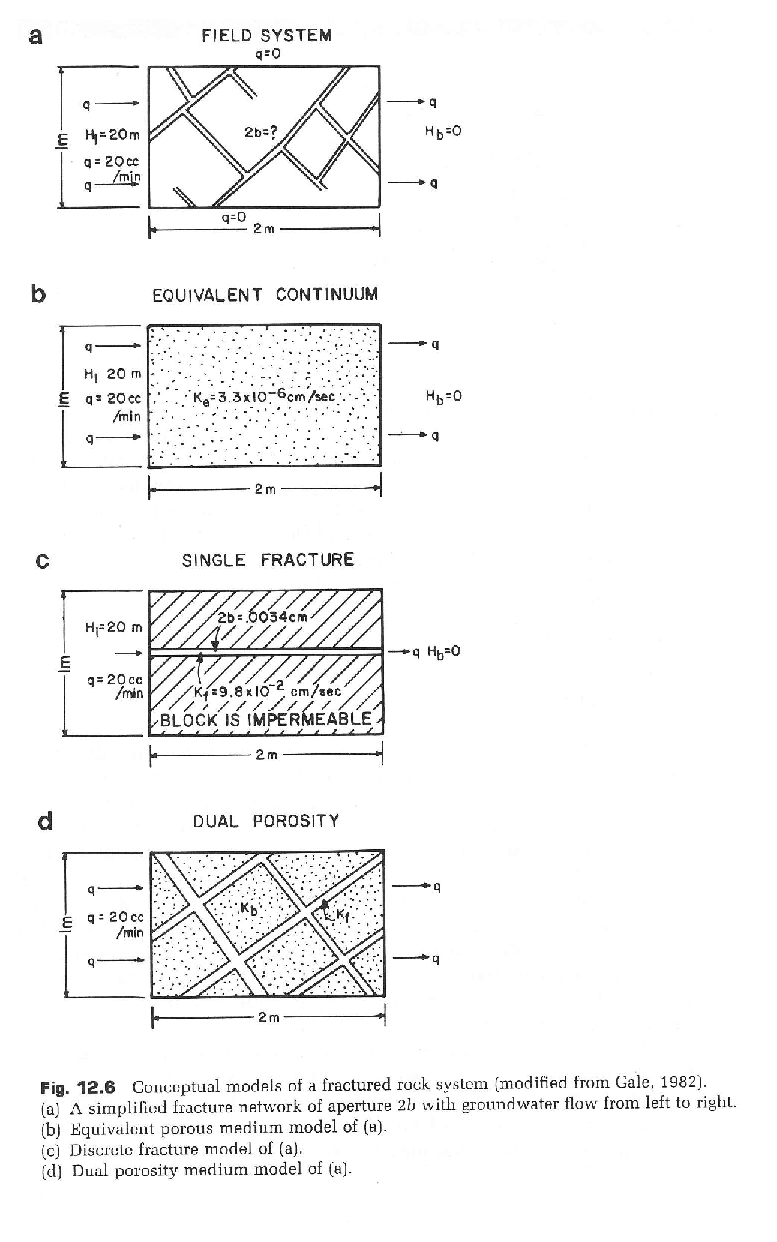
\includegraphics{./litrev/fractureModels.eps}
  \end{center}
  \caption{Various conceptual models may be used for the same natural system 
  \cite{anderson_applied_1992}.}
  \label{fig:fractureModels}
\end{figure}


The models arrived at via a continuum approximation are appropriate
for very fractured or very unfractured situations. This approximation is not 
suitable for situations in which the fracture width or frequency varies greatly.

Equivalent Porous Medium (EPM) models assert that a uniformly  fractured medium
can be approximated as a fractureless matrix with an effective porosity high
enough to account for real fracturation 
\cite{berkowitz_continuum_1988, anderson_applied_1992}.

Dual continuum models are the most widely employed models of fracture flow 
\cite{diodato_compendium_1994}. Dual Porosity Models make up one type of dual 
continuum model. This model incorporates advective
transport in simplistic, uniform fractures and diffusive sorption and
desorption into the stagnant (no advective transfer) water contained in the
pores of the rock matrix \cite{uleberg_dual_1996, ho_dual_2000}.


Dual Permeability Models are another type. These are similar to dual porosity
models, but incorporate advective transfer within the rock matrix and between
the rock matrix and the fracture volume\cite{uleberg_dual_1996, ho_dual_2000}.

\subsubsection{Discrete Fracture Network Models} 

Discrete fracture network models approximate that water and contaminants move 
only through the fracture network \cite{anderson_applied_1992, 
schwartz_fundamentals_2004}. Such an approximation is appropriate when flow 
through fractures is fast relative to porous flow. This modeling formulation 
is complex and requires detailed knowledge of the candidate lithology.

The flow in each fracture can be approximated, as in Schwartz and Zhang, with
the flow between two parallel plates having an aperture $b$, the mean fracture
height \cite{schwartz_fundamentals_2004}. For a fracture perpendicular to
gravitational acceleration, $g$, the hydraulic conductivity, $K$, is described
according to the cubic law as 

\begin{align} 
  K&= \frac{\rho_w g b^2}{12 \mu} \label{Kplates} 
  \intertext{where}
  \rho_w &= \mbox{ water density } [kg/m^3]\nonumber\\ 
  g &= \mbox{ gravitational acceleration } [m/s^2]\nonumber\\
  b &= \mbox{ plate aperture } [m]\nonumber\\
  \mu &= \mbox{ dynamic fluid viscosity } [kg/m\cdot s].\nonumber
\end{align}

Accordingly, the volumetric flow rate in the single fracture of width, $w$, can
be described in terms of the hydraulic head gradient, $\frac{\partial
h}{\partial L}$, as

\begin{align} 
  Q & = -Kbw\frac{\partial h}{\partial L}.
  \label{Qplates}
\end{align}

Calculation of the volumetric flow rate and corresponding solute transport in a
discrete fracture network model for many non-parallel fractures is an intensive
numerical computation. However, for uniformly fractured media, a fracture
network can be approximated by a set of parallel plates fractures. 

If flow is expect in the $\theta_f$ direction, and the fractures of the set are
spaced a distance, $d$, apart,

\begin{align} 
  N &= \mbox{fracture frequency}\nonumber\\ 
  &= \frac{cos(\theta_f)}{d}.  
  \label{fracfreq} 
\end{align}

The fracture network permeability is then defined as, 

\begin{align} 
  k_f =
\frac{b^3}{12N}.  
\label{fracperm} 
\end{align}

The permeability, $k$, in an equivalent permeability model is thereby obtained
by the permeabilities of the fracture network, $k_f$, and the permeability of
the host matrix, $k_m$. Following the derivation in Schwartz and Zhang, in
terms of the cross-sectional contact areas of the matrix and fractures $A_m$
and $A_f$, the equivalent permeability, $k$, can be expressed

\begin{align} 
  k = \frac{k_m + \frac{A_f}{A_m}k_f}{1+\frac{A_f}{A_m}}.
  \label{equivperm} 
\end{align}

This permeability is then used as the effective permeability of the rock in 
expressions that utilize it to determine the Darcy velocity, such as Equation 
\eqref{solperm}.

%\paragraph{Saturated Environments}

%\paragraph{Unsaturated Environments}


% The distribution of fracture aperture sizes in a saturated fractured hard rock 
% matrix determines the appropriate model with which to treat rock fracturation 
% and subsequent radionuclide transport through fracturous pathways. 

% Fracturation within a saturated medium can be treated either as an effective 
% porosity, in which n_eff is suggested according to the quantity of connected 
% fractures, much like connected pores, in a rock matrix. If these are of 
% similar sizes, 

% Fracturation in grantite, tuff, and basalt have a log normal distribution of 
% of fracture apertures. Therefore, there are a few large fractures but the 
% majority are microfractures.  Therefore, the equivalent porous medium approach 
% is inappropriate. Instead we must take the approach in which fractures of 
% larger aperture are given greater importance and are modeled as primary 
% conduits to the biosphere while minor fractures can be considered a part of 
% the porous medium of the saturated rock\cite{ahn_thesis}.


% For details about fracturation models in unsaturated rock, it's likely best to 
% consult YMR TSPA models.


%\paragraph{Diffusion Into Fracture}

%\paragraph{Advection Through Fracture}

%\paragraph{Effective Porosity}

%\paragraph{Major and Minor Fracturation}



%\subsubsection{Sudicky and Frind}
%
%%Sudicky and Frind give a model for fractured porous media that 
%analytically captures radionuclide mobility due to advection through 
%fractures as well as competing retardation factors including sorption on the 
%fracture walls, diffusion into stagnant fluid in the rock matrix, and 
%sorption into rock matrix walls. 

\section{Analytical Models of Heat Transport} \label{sec:analytical_heat}
 
A comprehensive model of a repository must arrive at an appropriate notion of 
heat-based repository capacity.  This requires a model which addresses heat 
transport through the repository as a function of spatial repository layout, 
waste stream decay heat, and heat transfer properties of the engineered barrier  
system and lithology. This model must sufficiently solve for peak temperatures 
at heat limited locations, which are in most cases at the waste package 
interface with the buffer material and the buffer material interface with the 
lithology. These heat limits were discussed in section 
\ref{subsec:claythermal}. 

Heat transfer in these concepts will be dominated by conductive  
heat transfer. In a closed system, very few air gaps will exist. For this 
reason,  heat transfer by radiation is likely to be negligible. Similarly, since  
water velocities are comparatively low, heat transfer by mass transfer or by 
convection will be small relative to conduction.  

A discussion of analytical models of heat transport follows that quantifies these 
modes of heat transfer and addresses their applicability to the model at hand. 

%%%%%%%%%%%%%%%% Analytical Heat Transport %%%%%%%%%%%%%%%%%%%%%%%%

\subsection{Conduction}

Conductive heat transfer occurs as a result of a temperature gradient. Heat 
flows diffusively from the hotter material to the cooler material over time and
steadily approaches thermal equilibrium. The general form of the conduction 
equation can be expressed


\begin{align}
  \nabla^2T + \frac{q'''}{k} = \frac{1}{\alpha}\frac{\partial T}{\partial t},
  \label{general}
  \intertext{which with no heat source becomes the transient Fourier equation,}
  \nabla^2T  = \frac{1}{\alpha}\frac{\partial T}{\partial t},
  \label{transfourier}
  \intertext{or to the Laplace equation in steady state,}
  \nabla^2T = 0.
  \label{laplace}
  \intertext{Replacing the source gives the steady state Poisson equation,}
  \nabla^2T + \frac{q'''}{k} = 0.
  \label{poisson}
\end{align}

An areal heat flux, $q'' [W/m^{2}]$ can be derived from an integration of  
Poisson's equation \eqref{poisson}  and expressed in terms of the thermal 
conductivity of the material, $k [W/m\cdot^{\circ}K]$, and the
temperature gradient $\nabla T [K/m]$ by the expression

\begin{align}
  q''= -k\nabla T.
  \label{fourier}
\end{align}

For the one dimensional case, equation \ref{fourier} can be reduced using a 
finite difference approximation. For a body at $x_1$ with temperature $T_1$
and a body with temperature $T_2$ at position $x_2$,

\begin{align}
  q_x'' &= -k_x\frac{dT}{dx}\\
  &=-k_x\frac{(T_1-T_2)}{x_1-x_2}.
\end{align}

\subsection{Convection}

Convective heat transfer occurs advectively in accordance with fluid movement. 
Convection can be expressed as

\begin{align}
  \dot{q} &= -hA\Delta T.
\end{align}

\subsection{Radiation}

Heat transfer by radiation is the result of the emission of electromagnetic 
waves. Planck black body radiation is analytically described, using $\sigma$, the   
Stefan-Boltzmann constant as

\begin{align}
  \dot{q} = \sigma A_1 F_{1\rightarrow 2}(T_1^4 - T_2^4)
  \label{planck}
  \intertext{where}
  \sigma =5.670373\times 10^{−8} [W/ m^{2} K^{4}]\nonumber
  \intertext{and}
  F_{1\rightarrow 2} =
  \begin{cases}
    \epsilon_1 &
    \mbox{ for a point source},\\
    \frac{1}{\frac{1}{\epsilon_1} + \frac{1}{\epsilon_2} - 1 } &
    \mbox{ for parallel plates},\\
    \frac{2\pi r_1 L}{\frac{1}{\epsilon_1} + \frac{1}{\epsilon_2} - 1 } \frac{r_1}{r_2} &
    \mbox{ for concentric cylinders}
  \end{cases}
  \intertext{where}
  \epsilon_i = \mbox{emissivity of surface i } [-]\nonumber\\
  r_i = \mbox{radius of cylinder i } [m] \nonumber\\
  L = \mbox{cylinder length }[m].\nonumber
\end{align}

\subsection{Mass Transfer}

Heat transfer by mass transfer is straightforward, resulting in the change in 
temperature in adjacent volumes as a result of matter movement. If the specific 
heat capacity of the transferred mass can be expressed as $c_p$, then the heat 
transfer is simply, 

\begin{align}
  \dot{q} = \dot{m}c_p\left( T_j - T_i \right)\\
  \intertext{where}
  c_p = \mbox{ specific heat capacity } [J/kg^{\circ}K].\nonumber
\end{align}

\subsection{Lumped Parameter Model}
\label{sec:lumpedparam}

The lumped heat capacitance model makes an analogy to electrical circuit by 
reducing a thermal system into discrete lumps. Such an approximation is 
appropriate when it can be assumed that the temperature gradient within each 
lump is approximately uniform. The appropriateness of this approximation can be
quantitatively expressed by comparison of the internal thermal resistance to the 
external thermal resistance. The Biot number, 

\begin{align}
  Bi = \frac{hA}{k}
  \label{biot}
\end{align}

indicates the relative speeds with which heat conducts within an object and 
across the boundary of that object. If the Biot number is low $(<0.1)$, and 
therefore conduction is faster within the object than at the boundary, the 
assumption of a uniform internal temperature is appropriate and the lumped 
parameter model may be expected to give a result within $5\%$ 
error\cite{incropera_fundamentals_2006}. This assists in choosing the size of 
distinct lumps within a conceptual model. 

The lumped capacitance model can address multiple media and multiple heat
transfer modes. The rate of heat transfer $\dot{q}\hspace{1mm}[Wm^{-2}K^{-1}s^{-1}]$ 
through a circuit is simply given as the quotient of the temperature 
difference and the sum of thermal resistances, $R_i [W\cdot K^{-1}]$,
of the multiple lumps 

\begin{align}
  \dot{q} = \frac{\Delta T}{\sum _{i=0}^{N}R_i}.
\end{align}

By representing the various modes of heat transport (i.e. conduction, 
convection, radiation, and mass transfer) with various expressions for 
resistance, the lumped capacitance model provides a solution to the transient 
problem described by the energy balance,

\begin{align}
  \left( \mbox{Energy added to body j in dt} \right) &= \left( \mbox{Heat 
  out of adjacent bodies into body j} \right)\nonumber\\
  c_j\rho_j V_j dT_j(t) &= \sum_{i=0}^{i=N}\left[\dot{q_{i,j}}\right]dt,
\end{align}

where $c_j\rho_jV_j$ is the total lumped thermal capacitance of the body.

For example, in the case of a simple convective circuit between two bodies, $i$ 
and $j$, the resistance of $j$ can be described as 
\begin{align}
  R_{conv} &= 1/hA
  \intertext{such that}
  c_j\rho_j V_j dT_j(t) &= \sum_{i=0}^{i=N}\left[ hA_j (T_i - T_j(t)) \right]dt.\\
\end{align}

A time constant appears under integration that describes the speed with which 
the body $i$ changes temperature with respect to the maximum temperature change,

\begin{align}
  \int_{T_j=T_0}^{T_j(t)} 
  \frac{dT_j(t)}{T_i-T_j}&=\frac{hA_j}{c_j\rho_jV_j}\int_0^t dt\\
  -ln\frac{T_i-T_j(t)}{T_i-T_0}&=\frac{hA_j}{c_j\rho_jV_j}t\\
  \frac{T_i-T_j(t)}{T_i-T_0}&= e^{-(hA_j/c_j\rho_jV_j)t}\\
  \intertext{such that}
  \frac{T_j(t)-T_i}{T_i-T_0}&= 1- e^{-t/\tau}\\
  \intertext{where}
  \tau &= \left( c_j\rho_jV_j/hA_j \right).
\end{align}

The time constant, $\tau$ is the time it takes for the body to change 
$(1-(1/e))\%\Delta T$ and is equal to the product of the thermal capacitance and 
thermal resistance of the body, $CR$, analogous to an electrical circuit.

\cite{el-wakil_nuclear_1981} This is the case for all resistances, $R_i$ 
representing modes of heat transfer. Thus, one can say, in general

\begin{align}
  \tau_j = c_j \rho_j V_j R_j.
\end{align}

\subsection{Impact of Repository Designs}

The repository layout has a significant influence on its heat limited capacity. 
Waste package spacing in drifts, boreholes, or alcoves, tunnel spacing, and
multiple gallery level designs can increase or decrease available heat loading. 
For example, in the \gls{YMR}, a variety of parameters have been shown to 
potentially increase the repository waste density. 

The \gls{YMR} statutory limit of once-through, thermal PWR waste is 70,000 tonnes 
SNF.  That is to say, the statutory line load limit is approximately 1.04 tonnes/m
for 67km of planned emplacement tunnels (with 81 meters between drifts). The
Office of Civilian Radioactive Waste Management Science and Engineering Report
gives this basic ``statutory limit'', but suggests an inherent design
flexibility that could allow for expansion. Multiple efforts have adjusted 
various repository layout parameters in order to develop expanded capacity 
models of the \gls{YMR}. Some of these efforts are detailed in Table 
\ref{tab:footprint}.

\begin{table}
  \centering
      \footnotesize{
      \begin{tabular}{|l|c|c|r|}
          \multicolumn{4}{c}{\textbf{Yucca Mounting Footprint Expansion Calculations}}\\
          \hline
          Author&Max. Capacity&Footprint&Details\\
          &$tonnes$&$km^2$&\\
          \hline
          &&&\\
          OCRWM&$70,000$&$4.65$&``statutory case''\\
          &$97,000$&$6$&``full inventory case''\\
          &$119,000$&$~7$&``additional case''\\
          \hline
          &&&\\
          Yim, M.S.&$75,187$&$4.6$&SRTA code\\
          &$76,493$&$4.6$&STI method\\
          &$95,970$&$4.6$&$63$m drift spacing\\
          &$82,110$&$4.6$&75 yrs. cooling\\
          \hline
          &&&\\
          Nicholson, M.&$103,600$&$4.6$&drift spacing\\
          \hline
          &&&\\
          EPRI&&&\\
          &$63,000$&$6.5$&Base Case CSNF\\
          option 1&$126,000$&$13$&expanded footprint\\
          option 2&$189,000$&$6.5$&multi-level design\\
          option 3&$189,000$&$6.5$&grouped drifts\\
          options 2+3&$252,000$&$6.5$&hybrid\\
          options 1+(2or3) &$378,000$&$13$&hybrid\\
          options 1+2+3 &$567,000$&$13$&hybrid\\
          \hline
        \end{tabular}
        \caption[Yucca Mountain Footprint Expansion Calculations]{Various analyses based on heat 
        load limited repository designs have resulted in footprint expansion calculations of the 
        YMR.} 
        }
      \end{table}
 

This inherent flexibility can come from an increase in the areal extent of the 
repository footprint, the density of drifts, or vertical expansion. The  ``full inventory'' Yucca
Mountain design alternative gives a maximum repository capacity of 97,000
tonnes. In addition, the current design for the repository has flexibility for
``additional repository capacity'' which would give a 119,000 tonne capacity at
1.04 tonnes/m.\cite{doe_yucca_2002} 

In addition to variable drift spacing, other modifications to repository layout
have had promising results in terms of heat-limited repository capacity. The
Electric Power Research Institute (EPRI) in their Room at the Mountain study
found that with redesign of the repository an increased capacity of at least
$400\%$ (295 tonnes once-through SNF) and up to $900\%$ (663 tonnes) could be
expected to be achieved. Proposed design changes include decreased spacing
between drifts, a larger areal footprint, vertical expansion into second and
third levels of repository space, and hybrid solutions involving combinations
of these ideas. In particular, EPRI suggests either an expansion of the
footprint with redesign of the current line load design plan or a
multi-level plan that repeats the footprint and line load design of the current
plan\cite{kessler_room_2006}.

%Specific Temperature Change analysis by Radel, Wilson, et al. find a maximum
%thermal capacity of 1.09 tonnes/m for commercial SNF (at an ELF of $49
%GWd_{th}/m$)\cite{radel_effect_2007}. 

Layout options such as age based fuel mixing also allows for decreases in drift 
spacing. In aged based fuel mixing, aged (long cool time) SNF is loaded in a 
mixture with young SNF. This age based fuel mixing has been shown to achieve a 
$48\%$ increase in the repository capacity as constrained by heat
load\cite{nicholson_thermal_2007}. This factor uses a fiducial default
footprint of $4.6 km^2$ used in the NRC TSPA.  The reported $48\%$ increase in
capacity results in total repository capacity of 103,600
tonnes\cite{williams_total_2001}.




\subsection{Heat Limits in Engineered Components} 

Various waste form constraints exist that limit fuel loading. These are 
in general less restrictive than heat limits resulting from geological medium 
constraints, however in some cases they are more restrictive. 

For example, the current constraining heat limit in borosilicated glass 
reported by the \gls{UFD} campaign is $500^{\circ}C$, corresponding to the 
temperature at which the glass can be expected to begin devitrifying 
\cite{carter_disposal_2010, hardin_generic_2011, soelberg_heat_2009}. For ceramic oxide 
fuel pellet waste forms, zirconium cladding has a heat limit of $350^{\circ}C$ 
to prevent rupture. 

\subsection{Specific Temperature Integral}

Linear mass loading ($tonnes/m$), linear thermal loading ($W/m$) and areal power 
density ($W/m^2$) are common metrics
for describing the loading of the repository. While these metrics are
informative for mass capacity and power capacity respectively, they fail to
reflect differences in thermal behavior due to varying SNF compositions.  A
closer look at the isotopics of the situation has proven much more applicable
to thermal performance studies of the repository, and the preferred method in
the current literature relies on specific temperature integrals.


Specific temperature integrals model the thermal source as linear along the
emplacement paths, similar to the line loading and areal power density metrics.
However, a temperate integral takes account of heat transfer behavior in the
rock, includes the effects of myriad SNF compositions, and gives the thermal
integration over time for any specific location within the rock.  Man-Sung Yim
calls this the Specific Temperature Increase method\cite{li_specific_2008}
though other researchers have other names for this method. Tracy Radel calls
her temperature metric at a point in the rock the Specific Temperature
Change\cite{radel_repository_2007}.

In a repository with linear drifts, the heat flux from the drifts can be
expressed as the superposition of the linear heat flux contributions of all the
radionuclides in the waste. The temperature change, more importantly can be 
expressed as a superposition of the temperature change contributions due to  
each radionuclide. Each radionuclide contributes in proportion to its
decay heat generation and its weight fraction of the SNF. With information
about isotopic composition of the SNF, the Specific Temperature Increase can
determine the maximum thermal capacity of the repository in terms of tonnes/m.
The length based accounting in $\frac{t}{m}$ is converted to
$\frac{t}{Repository}$ by multiplication with the total emplacement tunnel
length of the repository.  In the case of Yucca Mountain, this was 67 km.

\section{Detailed Computational Models of Radionuclide Transport}
\label{sec:detailed_radionuclide}

Detailed computational models of radionuclide transport seek to quantify the spatial 
movement of radionuclides within a repository environment due to heat 
generating waste forms. Such models are detailed with respect to their fine 
spatial and temporal resolution or with respect to the incorporation and 
coupling of numerous physical phenomena. Current detailed computational models 
addressing various repository geologies and geometries will be reviewed here 
that utilize finite differencing and finite element methods in many dimensions, 
sophisticated numerical solvers, and other high fidelity approaches.


\subsection{European RED-IMPACT} 

The RED-IMPACT assessment compared
results from European fuel cycle codes for various specific waste package
forms, radioactive and radiotoxic inventories, reprocessing discharges,  waste
package thermal power, corrosion of matrices, transport of radioisotopes and
resulting doses.  Granite, clay and salt were analyzed by various countries and 
codes as listed in table \ref{tab:red}.


%%%%%%%% RED-IMPACT Table %%%%%%%%%%%% 


\begin{table}
  \centering
  \footnotesize{
  \begin{tabular}{|l|c|c|c|c|}
    \multicolumn{5}{c}{\textbf{International Repository Concepts}}\\
    \hline
    Geology     & Nation      & Waste Stream   & Metric    & Institution \\
    \hline 
    Granite     & Spain       & HLW            & Heat Load & Enresa  \\
    Granite     & Czech Rep.  & HLW            & Heat Load & NRI \\
    Clay        & Belgium     & HLW            & Heat Load & SCK$\cdot$CEN \\
    Salt        & Germany     & HLW            & Heat Load & GRS \\
    Granite     & Spain       & HLW            & Dose      & Enresa  \\
    Clay        & Belgium     & HLW            & Dose      & SCK$\cdot$CEN \\
    Clay        & France      & HLW            & Dose      & CEA \\
    Salt        & Germany     & HLW            & Dose      & GRS  \\
    Granite     & Czech Rep.  & ILW            & LT Dose   & NRI  \\
    Granite     & Spain       & ILW            & LT Dose   & Enresa  \\
    Clay        & Belgium     & ILW            & LT Dose   & SCK$\cdot$CEN  \\
    Granite     & Spain       & HLW/ILW/Iodine & LT Dose   & Enresa \\
    Clay        & Belgium     & HLW/ILW/Iodine & LT Dose   & SCK$\cdot$CEN \\
    \hline
  \end{tabular}
  \caption[International Repository Concepts]{International repository concepts evaluated in the RED Impact 
  Assessment.\cite{von_lensa_red-impact_2008}}
  \label{tab:red}
  }
\end{table}




%%%%%%%%%%%%%%%%%%%%%%%%%%%%%%%%%%%%%%

%%%%%%%%%%%%%%%% Detailed Radionuclide Transport %%%%%%%%%%%%%%%%%%%%%%%%

\subsection{UFD Generic Performance Assessment Model}

The \gls{UFD} campaign is currently conducting an effort to produce
a \acrlong{GPAM} for analysis of {\glspl{GDSM} for various geological environments. 
Teams from \acrlong{ANL}, \acrlong{LBNL}, \acrlong{LANL}, and \acrlong{SNL} are developing
models of generic clay, granite, and salt disposal environments. Sandia is
simultaneously constructing a deep borehole disposal system model in crystalline 
rock. Each generic disposal system model will perform detailed calculations of 
radionuclide transport within its respective lithology 
\cite{clayton_generic_2011}. A 2012 goal of the 
project includes an overarching generic model that incorporates the various 
geologically distinct submodels in order to provide a fully generic repository 
model. This overarching \gls{GPAM} work will be incorporated into this effort.

The radionuclide transport calculations for the geologically distinct models 
are performed within the GoldSim simulation platform. GoldSim is a commercial 
simulation environment.
Probabilistic elements of the GoldSim modelling framework enable the models to 
incorporate \gls{FEPs} expected to take place probabilistically during the 
evolution of the repository \cite{clayton_generic_2011}.  

Cells within GoldSim represent components of the waste disposal system and
are linked by diffusive, advective, precipitated, direct, or  otherwise filtered
mass transfer links. 

Thermal modeling for the \glspl{GDSM} are conducted independently with 
associated codes capable of modeling thermal evolution for all geologies. For 
example, one thermal model is being created using the \gls{SINDAG} heat
transport solver and another is under development at \gls{LLNL} that utilizes 
a combination of MathCAD and Excel. 

\subsubsection{Clay/Shale GDSM}

The Clay \gls{GDSM} is being pursued by the team at \gls{ANL} and will be 
the primary model with which this work will conduct parametric regression 
analyses. 

The Clay \gls{GDSM} models a single waste form, waste package, \gls{EBS}, 
\gls{EDZ}, and far field zone. This waste unit cell is modeled with boundary 
conditions such that it may be repeated throughout the extent of a repository 
configuration. 

The waste form and engineered barrier system are modeled as well-mixed volumes 
and radial transport away from the cylindrical base case unit cell is modeled as  
one dimensional.

Two radionuclide release pathways are considered. One is the nominal, undisturbed 
case, while the other is a fast pathway simulating a disturbed case
\cite{clayton_generic_2011}.


\subsubsection{Granite GDSM}

\gls{LANL} and \gls{SNL} have created a model of the granite repository concept  
in a saturated, reducing environment.

Waste form degradation is modeled as a constant, fractional rate to represent 
dissolution for both canonical borosilicate glass and commercial used fuel 
waste forms.  

Though waste package failure is conservatively assumed to be instantaneous,
waste package release into the near field is solubility limited as is the near 
field to far field interface. 

Transport through the buffer is modeled as entirely diffusive coupled with 
sorption. Advection is neglected.

The far field was represented using a model that includes advection, diffusion 
and sorption. Specifically, the \gls{FEHM} code was coupled into GoldSim to 
represent the far field.

\subsubsection{Salt GDSM}

The salt repository concept has an alcove gallery geometry and is located in a 
bedded salt formation. The formation is located in a reducing, saturated 
environment. Once waste packages  are horizontally placed in a corner of the 
alcove, the space is backfilled with crushed salt. 

Decay heat induced salt consolidation and brine flow are primary focuses of 
this analysis and inform radionuclide transport calculations. 

A constant, temperature independent annual degradation rate model is used to 
represent waste form dissolution for both canonical borosilicate glass and 
commercial used fuel waste forms. Waste package failure is conservatively 
assumed to be instantaneous, and all near field components are modeled as a 
single mixed cell, the water volume of which is determined by the bulk volumes 
and degraded porosities of contained materials (e.g. bentonite buffer). A block  
of rock below the salt provides the pathway interface to an aquifer below. 
Radionuclide transport into that interface is modeled as diffusive, advective, and 
solubility limited.

The far field is modeled using an equilibrium sorption model in addition 
to solubility limited diffusion and advection. In such an equilibrium sorption 
model, the sorption to precipitation balance is assumed to be at a 
reaction equilibrium. In this way, the partitioning coefficient $K_d$ is used to 
quantify the ratio between dissolved and undissolved reactant. Radionuclide transport
in the far field takes place for 5km, and ends in a biosphere model. 

Two radionuclide release pathways are considered. One is the nominal, undisturbed 
case, which the other is a fast pathway simulating a disturbed case
\cite{clayton_generic_2011}.


\subsubsection{ Deep Borehole GDSM}

The deep borehole model concept consists of some 400 waste canisters in a 5km 
deep hole within a low permeability, high salinity region characteristic of 
crystalline rock formations at depth. The lower 2km of the hole are filled 
by waste packages as well as spacing and sealing plugs. A 1km sealing zone 
extends above the waste disposal region.

As with the salt model, a constant, temperature independent annual degradation
rate model is used to represent waste form dissolution for both canonical 
borosilicate glass and commercial used fuel waste forms. Waste package failure 
is conservatively assumed to be instantaneous.

Flow in the vicinity of the borehole was modeled using tabulated groundwater 
flow velocities obtained from simulations run using the \gls{FEHM} code 
meshed in three full dimensions with the \gls{CUBIT} meshing tool 
\cite{clayton_generic_2011}.

\subsection{Li Model\cite{li_methodology_2006}} As a function of time, water
enters the Engineered Barrier System and corrodes the waste packages.  These
fail and from the failed waste packages radionuclides are released according to
advective transfer.  Further transport through the near and far field rock
medium is modeled in two modes, one representing the Unsaturated Zone, and one
representing the Saturated Zone.

Waste package failure and radionuclide release are modeled with two TSPA
code modules called EBSFAIL and EBSREL. The waste package failure rate is
determined from EBSFAIL, which incorporates waste form chemistry, humidity,
oxidation, etc and upon contact from water begins the degradation process. The
results of EBSFAIL become the input to EBSREL, which models corresponding
radionuclide release from those failed waste packages. Mass balance governing the
radionuclide release rate in this model allows advective transfer to dominate and
takes the form:

\begin{equation}
\dot{m_i}=w_{li}(t)-w_{ci}{t}-m_i\lambda_i+m_{i-1}\lambda_{i-1}.\nonumber
\end{equation}

In this expression, $w_{li}(t)$ is the rate $[mol/yr]$ of isotope \emph{i}
leached into the water.  It is a function of water flow rate, chemistry, and
isotope solubility. $m_i$ describes the mass of isotope \emph{i}, and
$\lambda_i$ $[s^{-1}]$ describes its decay constant. Finally, $w_{ci}(t)$
describes the advective transfer rate $[mol/yr]$ of the isotope \emph{i}. This 
model defines $w_{ci}$ as:

\begin{equation}
  w_{ci}(t)=C_i(t)q_{out}(t). 
\end{equation}

where $q_{out}$ is the volumetric flow rate of the water $[m^3/yr]$, and 
$C_i$ is the concentration on isotope $i$ in the waste package volume 
$m_i/V_{wp}$ in $[mol/m^3]$. These assumptions fail to take into account any
differences in the varying solubilities of the isotopes, but are quite
sensitive to the concentration of an isotope \emph{i} in the waste package
volume.  

\subsection{ANDRA Dossier 2005} The ANDRA Dossier 2005 studies provided
detailed radionuclide transport calculations for both argillaceous clay and granite
formations. 

\subsubsection{ANDRA Clay Model} 

In the \gls{ANDRA} clay model, complicated saturation and resaturation phenomena 
are neglected and it is assumed that the initial repository condition is fully
resaturated. This is a conservative simplification. Another conservative
assumption is one in which the evacuation disturbed zone does not heal. Rather,
it is modeled in its damaged state immediately after excavation. 

This model only tracks 15 radionuclides of importance.  These are chosen to be those
with halflives over 1000 years and most toxicity or mobility
\cite{andra_argile:_2005}. The behavior of radionuclides in 
glassvitrification forms can be summarized by categorizing them into mobile,
intermediate, and well retained elements. 

Some specific codes and the method with which they were used in the \gls{ANDRA} 
clay assessment are listed in Table  \ref{tab:andra}.

%%%%%%%%%%%%%%%%%%%%%%%%%%%%%%%%%%%%%% 
%%%%%% Andra Sub-Codes Table %%%%%%%%%
%%%%%%%%%%%%%%%%%%%%%%%%%%%%%%%%%%%%%% 

\begin{table}
\centering
\footnotesize{
\begin{tabular}{|l|l|}
  \multicolumn{2}{c}{\textbf{Detailed Nuclide Transport Models Used in the ANDRA analysis.}}\\
\hline
Models &                                          Codes\\
\hline
Hydrogeology and particle tracking      &  Connectflow (3D finite element)\\
in continuous porous media              &  Geoan (3D finite differences).\\
                                        &  Porflow (3D finite differences).\\
Hydrogeology and particle tracking      &  Connectflow (3D finite elements).\\
in discrete fracture networks.          &  FracMan (discrete fracture networks) and\\
                                        &  MAFIC (3D finite elements).\\
Transport in continuous porous media.   &  PROPER (finite differences),\\
                                        &  Goldsim (control volumes), and\\ 
                                        &  Porflow (control volumes?).\\
Transport in discrete fracture networks.&  PROPER (1D stream tube concept).\\
                                        &  PathPipe (networks of tubes)\\
                                        &  and Goldsim (networks of 1D pipes).\\
\hline
\end{tabular}
\caption[Particle Transport Codes Used in ANDRA Assessment]{Similar to the Total System Performance Assessment, ANDRA's analyses are a coupled mass of many codes. Table reprouced from Argile Dossier 2005 \cite{andra_argile:_2005}}
\label{tab:andra}
}
\end{table}


%%%%%%%%%%%%%%%%%%%%%%%%%%%%%%%%%%%%%%

%more details in inset 10-2, andra argile phenom. . 

%%%%%%%%%%%%%%%%% From Andra %%%%%%%%%%%% 
% mobile elements. They comprise the alkalis (sodium, lithium), molybdenum and 
% technetium. They are released congruently with the degradation of the vitreous 
% matrix. (Andra, 2005d). Of the chemical toxins, boron corresponds to this 
% category of elements.  

%intermediate elements are partially retained in the alteration layer when the 
%glass degrades. These elements are caesium, alkaline earth metals (calcium, 
%strontium, barium), silicon and aluminium (Andra, 2005d).


%Highly retained elements are insoluble at the basic pH imposed by the

%degradation of the glass. They include all the transition elements (iron, 
%nickel, zinc, zirconium, etc.) and lanthanides and actinides (Andra, 2005d ; 
%Fillet, 1987).  
%%%%%%%%%%%%%%%%%%%%%%%%%%%%%%%%%%%%%%%%%


Waste form dissolution and package release was assumed to be immediate for some
waste forms and corrosion rate based for those where appropriate data was
available. Vitrified waste package releases were either modeled with a simple
model or a two phase phenomenological model. 

%(pg198 for references to themath)

Transpor through the backfill is modeled as diffusive, with high permeability 
after degradation.  The evacuation disturbed zone has both a fracture zone and a 
microfissure zone.  In the host formation, movement is dominated by diffusion, 
and advection is modeled, but is negligible.

%advection dispersion equation is developed in the section entitled ``The 
%retention and transport of solutes.'' inset 10-11 gives solubility and sorption 
%values for important elements.


% from andra pg 202: 
% 
%The permeability values determined in situ or on undisturbed samples are 
%between 10-14 and 10-13 m/s. The structure of the medium suggests permeability 
%anisotropy and leads to cautiously adopting a value ten times higher for the 
%horizontal permeability.  The reference calculation therefore takes into 
%account a vertical permeability value of 5.10-14 m/s and a horizontal 
%permeability value of 5.10-13 m/s. The influence of temperature on the 
%permeability value is not included in calculations for the normal evolution 
%scenario, but it is taken into account in the altered evolution scenarios 
%because of its greater influence.  

Tools used in the ALLIANCES software platform include Castem, PorFlow and Trace
for hydraulic calculations and radionuclide transport and Prediver and Colonbo for
waste package failure.



%\subsection{SKB Model} 
%\gls{SKB} used ConnectFlow to model Forsmark particle
%transport. It also used a model called MIKE SHE in conjunction with ConnectFlow
%in order to model ``uses locally measured meteorological data to simulate
%transient water flow in the saturated (groundwater) and unsaturated zones,
%overland flow, and water losses due to evapotranspiration processes
%(interception, evaporation and transpiration)''. CF contains an elaborate
%description of flow within the rock, whereas the MS model provides more
%detailed information on near-surface water flow paths and the associated
%discharge paths.



\section{Detailed Computational Models of Heat Transport}
\label{sec:detailed_heat}

%%%%%%%%%%%%%%%% Detailed Heat Transport %%%%%%%%%%%%%%%%%%%%%%%%

Detailed heat transport models seek to quantify the heat evolution within a 
repository environment due to heat generating waste forms. Such models are 
detailed with respect to their detailed spatial and temporal resolution or 
with respect to the incorporation and coupling of numerous physical phenomena. 
Such codes typically utilize finite differencing or finite element methods in 
many dimensions or sophisticated numerical solvers, respectively. 



\subsection{Bauer SINDA{\textbackslash}G Model}

This model, created at Argonne National Lab by Ted Bauer uses the \gls{SINDAG} 
lumped capacitance solver. Originally created for optimal waste loading analysis 
of the \gls{YMR}, the Bauer model is geometrically adjustable in two dimensions,   
as is demonstrated in Figure \ref{fig:sindageom}. The tunnel size is a fixed 
parameter in the model, but the optimal drift spacing for a particular waste 
stream and package loading is solved for with an optimization loop within this 
model.

\begin{figure}[htbp!]
  \begin{center}
    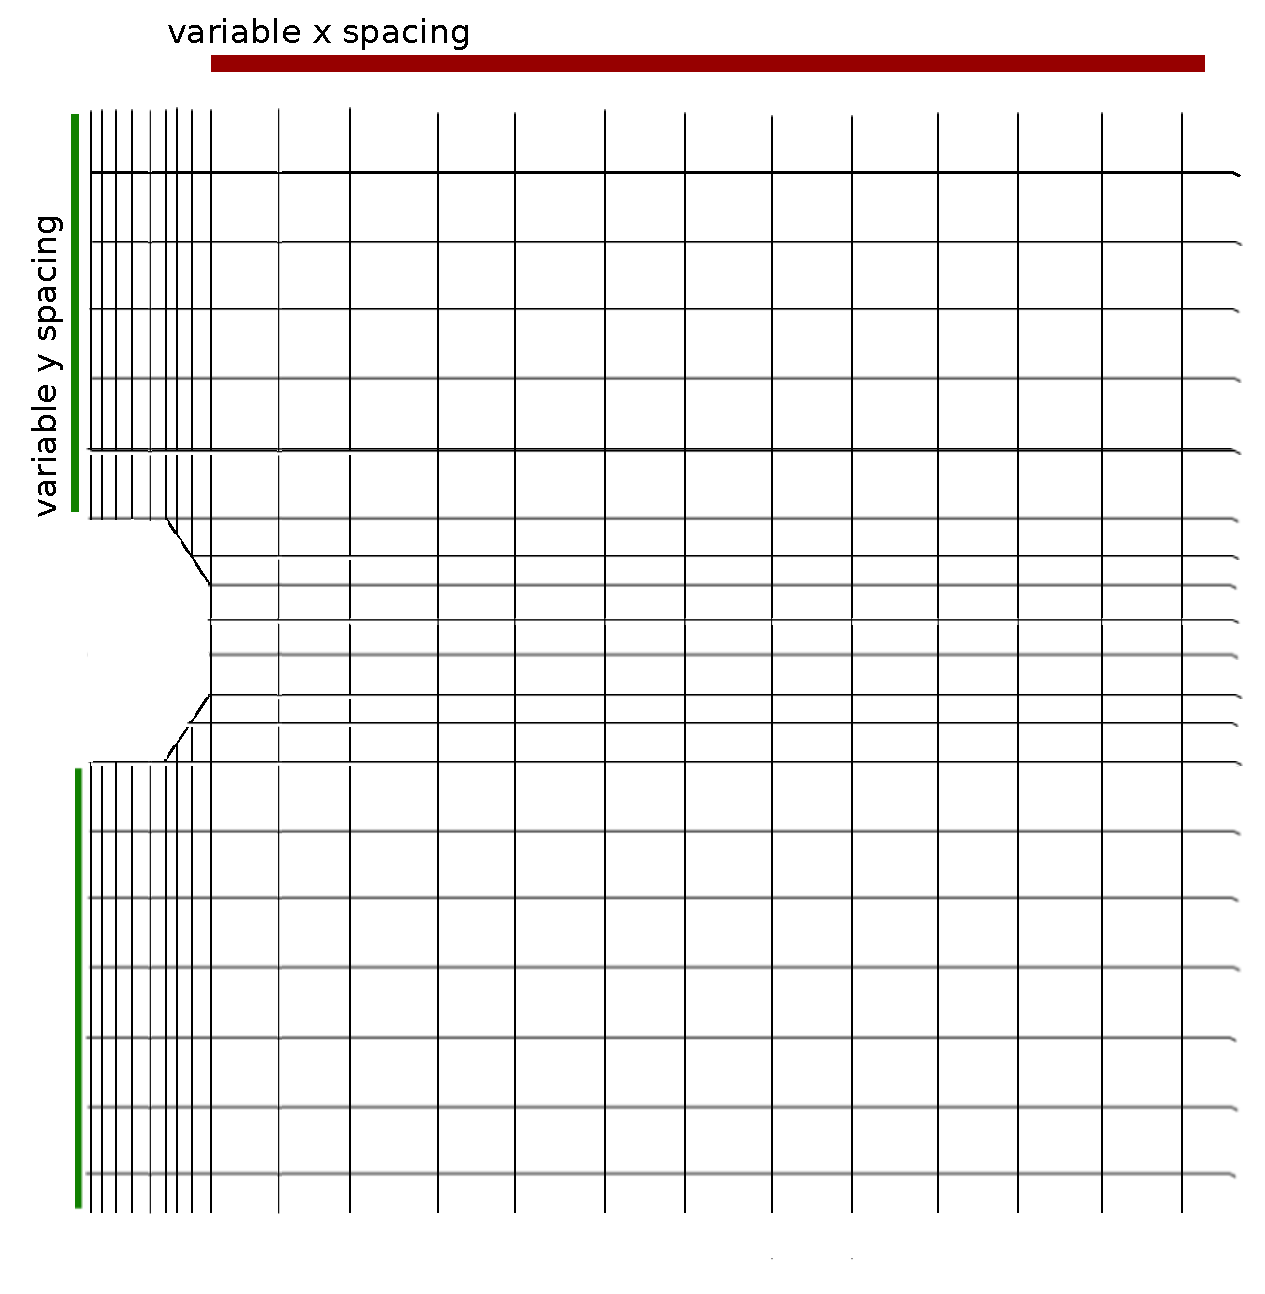
\includegraphics[height=10cm]{./chapters/current/sindageom.eps}
  \end{center}
  \caption{The geometry of the thermal model can be adjusted in two dimensions, 
  altering the tunnel spacing and the vertical distance from the aquifer.}
  \label{fig:sindageom}
\end{figure}

The \gls{SINDAG} lumped capacitance solver solves a thermal circuit, for which 
conducting nodes may be of four types corresponding to the four modes of heat 
transfer. Nodes are connected by conduction, convection, radiation, and mass 
flow heat transfer links. As discussed in section \ref{sec:lumpedparam}, these 
are represented by

\begin{align}
  R_{cond} &= \frac{L}{k A}\\
  R_{conv} &= \frac{1}{h A}\\
  R_{mf}  &= \frac{1}{\dot{m}c_p}\\
  R_{rad}  &= \frac{1}{\sigma F_{ij}A\left[ T_i + T_A + T_j + T_A 
  \right]\left[(T_i+T_A)^2+(T_j+T_A)^2\right]}
  \intertext{where}
  k&= ~~\mbox{conductivity}[W\cdot m^{-1}\cdot K^{-1}]\nonumber\\
  A&= ~~\mbox{area} [m^2]\nonumber\\
  c_p&=~~\mbox{specific heat capacity} [J\cdot K^{-1}]\nonumber  \\
  h&= ~~\mbox{heat transfer coefficient}[W\cdot m^{-1} \cdot K^{-1}\nonumber \\
  \dot{m}&= ~~\mbox{mass transfer rate}[kg\cdot s^{-1}]\nonumber \\
  T_i&= ~~\mbox{lump temperature} [^{\circ}C] \nonumber\\
  T_A&= ~~\mbox{absolute temperature} [^{\circ}C] \nonumber\\
  F_{ij}&= ~~\mbox{radiation interchange factor} [-] .\nonumber
\end{align}

With these representations of thermal resistance, a lumped parameter model will 
require an analysis that determines the appropriate length scale for the lumped 
parameter approximation.

Given one or more heat constraints, the Bauer model  optimizes 
spatial waste loading in order to meet those constraints with maximal waste 
loading. For example, given a constraint at the edge of the waste package, the 
model utilizes the \gls{SINDAG} lumped capacitance solver to determine the two 
dimensional heat evolution of the repository as a result of a given waste package 
composition for various drift spacings and arrives at an ideal drift spacing by 
iteration.


\subsection{LLNL MathCAD Model}

This model, created at \gls{LLNL} for the \gls{UFD} campaign, is written in a 
combination of MathCAD and Excel. The model consists of two physical parts, the  
first is the host rock, and the second models the waste form, package, and buffer 
as a single \gls{EBS} unit. Since the thermal mass of the \gls{EBS} is small in
comparison to the thermal mass of the host rock, it may be treated as quasi-steady
state. Thus, the transient state of the transient temperature between the host
rock and the EBS can be found with a MathCAD solution of the transient homogeneous 
conduction equation,

\begin{align}
  \nabla^2T  = \frac{1}{\alpha}\frac{\partial T}{\partial t}.
  \label{condGl}
\end{align}

Superimposed point and line source solutions allow for a notion of the repository 
layout to be modeled in the host rock. The solution of this equation at the 
boundary of the EBS and the waste package is then treated as a boundary condition 
for the heterogeneous steady state equation, 

\begin{align}
  \dot{q} &= U A_{out} \left( T_{in} - T_{out} \right)
  \label{condGeneral}
  \intertext{where}
  U&=\frac{1}{\sum_{i}R_i}
  \intertext{which, for the detailed EBS becomes}
  U&=\frac{1}{R_{WF}+R_{WP}+R_{buffer}+\cdots}
\end{align}

which calculates a resulting temperature gradient through the geometry at each 
point in time for each layer surface, assuming an infinite line source 
\cite{hardin_generic_2011}.

The process is then iterated with a one year resolution in order 
to arrive at a heat evolution over  the lifetime of the repository. This model 
seeks to inform heat limited waste capacity calculations for each geology, for 
many waste package loading densities, and for many fuel cycle options.  



\subsection{Other Numerical Methods}

Codes used by repository modeling efforts investigated in this review include 
finite difference codes, finite element codes, and specific temperature 
integrals.  Some efforts and their methods are listed in Table \ref{tab:heat}.


%%%%%%%%%%%%%%%%%%%%%%%%%%%%%%%%%%%%%%%%%%%%%%%% 
%%%%% Heat Load Computational Models Table %%%%% 
%%%%%%%%%%%%%%%%%%%%%%%%%%%%%%%%%%%%%%%%%%%%%%%% 

 \begin{table}
    \centering
    \footnotesize{
    \begin{tabular}{|l|c|c|l|}
      \multicolumn{4}{c}{\textbf{Models of Heat Load for Various Geologies}}\\
      \hline
      Source & Nation & Geology & Methodology \\  
      (Who) & (Where) & (What) & (How) \\  
      \hline
      Enresa \cite{von_lensa_red-impact_2008}           & Spain       & Granite       &  CODE\_BRIGHT  \\ 
      NRI   \cite{von_lensa_red-impact_2008}            & Czech Rep.  & Granite       &  Specific Temperature Integral   \\
      ANDRA \cite{andra_granite:_2005}                  & France      & Granite       &  3D Finite Element CGM code   \\
      SKB \cite{ab_long-term_2006}                      & Sweden      & metagranite   &  Forsmark / Laxemar Site \\
                                                        &             &               &  Descriptive Model (SDM)\\
      SCK$\cdot$CEN   \cite{von_lensa_red-impact_2008}  & Belgium     & Clay          &  Specific Temperature Integral   \\ 
      ANDRA \cite{andra_argile:_2005}                   & France      & Argile Clay   &  3D Finite Element CGM code   \\
      NAGRA \cite{johnson_project_2002, johnson_calculations_2002}  & Switzerland  & Opalinus Clay &  3D Finite Element CGM code \\
      GRS \cite{von_lensa_red-impact_2008}              & Germany     & Salt          &  HEATING (3D finite difference)   \\ 
      NCSU(Li)   \cite{li_examining_2007}               & USA         & Yucca Tuff    &  Specific Temperature Integral \\        
      NCSU(Nicholson) \cite{nicholson_thermal_2007}     & USA         & Yucca Tuff    &  SRTA and COSMOL codes\\
      Radel \& Wilson \cite{radel_repository_2007}      & USA         & Yucca Tuff    &  Specific Temperature Change \\ 
      \hline
    \end{tabular}
    \caption[Models for Heat Transport for Various Geologies]{Methods by which to calculate heat 
    load are independent of geology. Maximum heat load constraints, however, vary among host formations. }
    \label{tab:heat}
    }
  \end{table}


%%%%%%%%%%%%%%%%%%%%%%%%%%%%%%%%%%%%%%



